%%%%%%%%%%%%%%%%%%%%%%%%%%%%%%%%%%%%%%%%%
% This document provides a sample senior
% thesis proposal template for use
% by Allegheny's Computer Science majors.
%
% This template was adopted from Jeremie Gillet
% Ref: https://github.com/oist/LaTeX-templates
%
% Author: Janyl Jumadinova
% Last Updated: November 15, 2020
%
%%%%%%%%%%%%%%%%%%%%%%%%%%%%%%%%%%%%%%%%%

%----------------------------------------------------------------------------------------
%	PACKAGES AND OTHER DOCUMENT CONFIGURATIONS
%----------------------------------------------------------------------------------------

\documentclass[12pt,oneside]{book} % 12 pt font, one-sided book style
\usepackage[a4paper, includehead, headheight=0.6cm, inner=3cm ,outer=2.5cm, top=2.5 cm, bottom=2.5cm]{geometry}  % Changing size of document
\usepackage[english]{babel} % The document is in English
\usepackage[utf8]{inputenc} % UTF8 encoding
\usepackage[T1]{fontenc} % Font encoding

\usepackage{listings}
\usepackage{color}

\definecolor{dkgreen}{rgb}{0,0.6,0}
\definecolor{gray}{rgb}{0.5,0.5,0.5}
\definecolor{mauve}{rgb}{0.58,0,0.82}

\lstset{frame=tb,
  language=Java,
  aboveskip=3mm,
  belowskip=3mm,
  showstringspaces=false,
  columns=flexible,
  basicstyle={\small\ttfamily},
  numbers=none,
  numberstyle=\tiny\color{gray},
  keywordstyle=\color{blue},
  commentstyle=\color{dkgreen},
  stringstyle=\color{mauve},
  breaklines=true,
  breakatwhitespace=true,
  tabsize=3
}

\usepackage{graphicx} % For including images
\graphicspath{{./images/}} % Specifies the directory where images are stored

\usepackage[table, xcdraw]{xcolor}
\usepackage{smartdiagram}
\usepackage{longtable} % tables that can span several pages
\usepackage[bf]{caption} % caption: FIG in bold
\usepackage{fancyhdr} % For the headers

\newcommand{\numberedchapter}{ % Preparation for numbered chapters
	\cleardoublepage % To make sure the previous headers are passed
	\fancyhead[RE]{{\bfseries \leftmark}}% Headers for left pages
	\fancyhead[LO]{{\bfseries \rightmark}}}% Headers for right pages
\newcommand{\unnumberedchapter}[1]{ % Preparation for unnumbered chapters
	\cleardoublepage % To make sure the previous headers are passed
	\addcontentsline{toc}{chapter}{#1} % Also adds the chapter name to the Contents
	\fancyhead[RE]{{\bfseries #1}} % Headers for left pages
	\fancyhead[LO]{}}%Headers for right pages

\usepackage{emptypage} % No headers on an empty page

\usepackage{eso-pic} % For the background picture on the title page
\newcommand\BackgroundPic{%
\put(0,-120){%
\parbox[b][\paperheight]{\paperwidth}{%
\vfill
\centering

\includegraphics[width=4in]{images/logo}%
\vfill
}}}

\usepackage{hyperref} % Adds clickable links at references

%----------------------------------------------------------------------------------------
%	ADD YOUR CUSTOM VALUES, COMMANDS AND PACKAGES
%----------------------------------------------------------------------------------------

% Open preamble/mydefinitions.tex and enter some values (name, thesis title...)
% and include your own custom LaTeX functions and packages


%----------------------------------------------------------------------------------------
% values for the proposal
%----------------------------------------------------------------------------------------

\newcommand{\name}{Jordan Wilson} % Author name
\newcommand{\thesistitle}{Assessing vulnerabilites using SQL injection} % Title of the thesis
\newcommand{\submissiondate}{\today} % Submission date "Month, date year"
\newcommand{\supervisor}{Oliver Bonham-Carter} % First reader's name
\newcommand{\cosupervisor}{Douglas Luman} % Second reader's name


%----------------------------------------------------------------------------------------
%	BIBLIOGRAPHY STYLE
%----------------------------------------------------------------------------------------


\bibliographystyle{acm}

%----------------------------------------------------------------------------------------
%	YOUR PACKAGES (be careful of package interaction)
%----------------------------------------------------------------------------------------

\usepackage{amsthm,amsmath,amssymb,amsfonts,bbm}% Math symbols
\usepackage{listings}
\usepackage{color}
%----------------------------------------------------------------------------------------
%	YOUR DEFINITIONS AND COMMANDS
%----------------------------------------------------------------------------------------

% New Commands
\newcommand{\bea}{\begin{eqnarray}} % Shortcut for equation arrays
\newcommand{\eea}{\end{eqnarray}}
\newcommand{\e}[1]{\times 10^{#1}}  % Powers of 10 notation


\begin{document}

%----------------------------------------------------------------------------------------
%	TITLE PAGE
%----------------------------------------------------------------------------------------

\pagestyle{empty} % No page numbers
\frontmatter % Use roman page numbering style (i, ii, iii, iv...) for the preamble pages

\begin{titlepage}
\AddToShipoutPicture*{\BackgroundPic}
\begin{center}
\vfill
{\large \scshape Allegheny College \\ Department of Computer Science }\\[1.4cm]
{\Large Senior Thesis}\\[0.5cm]
\rule{\textwidth}{1.5pt}\\[0cm]
{\huge \bfseries \thesistitle \par \ }\\[-0.5cm]
\rule{\textwidth}{1.5pt}\\[2.5cm]
\hfill  by\\[1cm]
\hfill  {\large \bfseries\name}\\
\vfill
{\hfill \large Project Supervisor: \textbf{\supervisor}} \\
\ifx\cosupervisor\undefined\else{\hfill \large Co-Supervisor: \textbf{\cosupervisor}} \\ \fi
\vspace{1cm}
\hfill  \submissiondate
\end{center}
\end{titlepage}


\pagestyle{fancy} % Changes the headers
\fancyhf{}% Clears header and footer
\fancyhead[RO,LE]{\thepage} % page number on the outside of headers

%-------------------------------------------------------------------------------
%	PREAMBLE PAGES (delete unnecessary pages)
%   preamble pages besides abstract are optional
%-------------------------------------------------------------------------------

\unnumberedchapter{Abstract} 
\chapter*{Abstract} 

In this thesis, I will attempt to perform a SQL injection attack on a web application. In our current times, technology is moving rapidly and it is proving to shape our society and our future. A big concern with this is the idea of security and how important that role plays in protecting our data and what we are doing. SQL injection is a tool that is going to teach me just how important the role of security plays and how I may effectively understand how people are being able to retrieve data. Security is certainly a big issue in our society as some of the biggest companies in our country are being hacked. This certainly is not something the companies want happening and it is not what the customers of the company want happening either as it is their information that is being leaked. With the knowledge and information I gain, I hope to be able to better figure out why this type of vulnerability might be so common but to also create a prototype in hopes that it could defend against this type of vulnerability. The problem is that there are other types of vulnerabilities out there as well so being able to be completely safe from all of them is a bit difficult but with the idea of my prototype I hope to shed some light to help mitigate one vulnerability so we can continue to slowly mitigate more of them. SQL injection is certainly a controversial topic as people have used it for harm in the past, but with proper understanding, developers can put in place proper security measures to safeguard against the attack.
\unnumberedchapter{Acknowledgment} 
\chapter*{Acknowledgment} 

First and foremost, I have to thank my research supervisors, Professor Oliver Bonham-Carter, and Professor Douglas Luman. Without their assistance and dedicated involvement in every step throughout the process, this paper would have never been accomplished. I would like to thank you very much for your support and understanding over these past few months. 

\bigskip

I would also like to thank all of the professors at the Allegheny College Computer Science department including Professors Oliver Bonham-Carter, Douglas Luman, Janyl Jumadinova, Gregory Kapfhammer, and Aravind Mohan. Their teaching styles and enthusiasm helped me find my passion for what I wanted to do as well as teach me how to design, execute, analyze and interpret code throughout the entire computer science discipline.

\bigskip

Last but certainly not least, I would like to thank my family as well. A big shoutout to my brother for helping me execute my research and proposed idea. Without him, I would not have been able to accomplish a lot of my work.


\unnumberedchapter{Abbreviations} 
\chapter*{Abbreviations} 

\begin{longtable}{rl}
API & application programming interface\\
CSV & comma separated values\\
Daas & data as a service\\
DMZ & Demilitarized zone\\
DNS & domain name system\\
DSL & digital subscriber line\\
GUI & graphical user interface\\
Haas & hardware as a service\\
HTML & hypertext markup language\\
Iaas & infrastructure as a service\\
IKE & internet Key Exchange\\
ISDN & integrated services digital network\\
ISP & internet service provider\\
LAMP & linux, apache, mysql, and php\\
LAN & local area network\\
PHP & hypertext preprocessor\\
PKI & public key infrastructure\\
Qos & quality of service\\
Saas & software as a service\\
SQL & structured query language\\
SSH & secure shell\\
URL & uniform resource locator\\
VPN & virtual private network\\
XSS attacks & cross site scripting\\
\end{longtable}

%-------------------------------------------------------------------------------
%	LIST OF CONTENTS/FIGURES/TABLES
%-------------------------------------------------------------------------------

\unnumberedchapter{Contents}
\tableofcontents % Write out the Table of Contents
\unnumberedchapter{List of Figures}
\listoffigures % Write out the List of Figures
\unnumberedchapter{List of Tables}
\listoftables % Write out the List of Tables

%-------------------------------------------------------------------------------
%	THESIS MAIN TEXT
%-------------------------------------------------------------------------------

\addtocontents{toc}{\vspace{2em}} % Add a gap in the Contents, for aesthetics
\mainmatter % Begin numeric (1,2,3...) page numbering

%----------------------------------------------------------------------------------------
%	START DELETE TEXT
%----------------------------------------------------------------------------------------

%----------------------------------------------------------------------------------------
% STOP DELETE
%----------------------------------------------------------------------------------------

%\numberedchapter{Introduction} % Title of the numbered chapter
\definecolor{dkgreen}{rgb}{0,0.6,0}
\definecolor{gray}{rgb}{0.5,0.5,0.5}
\definecolor{mauve}{rgb}{0.58,0,0.82}

\lstset{frame=tb,
  language=Java,
  aboveskip=3mm,
  belowskip=3mm,
  showstringspaces=false,
  columns=flexible,
  basicstyle={\small\ttfamily},
  numbers=none,
  numberstyle=\tiny\color{gray},
  keywordstyle=\color{blue},
  commentstyle=\color{dkgreen},
  stringstyle=\color{mauve},
  breaklines=true,
  breakatwhitespace=true,
  tabsize=3
}





\chapter{Introduction}



\section{Motivation}
\label{sec:motivation}

In this day in age, technology is continuing to rapidly grow and expand. It is expected in 2020 that there will be two-hundred billion devices connected \cite{Milkovich:2013}.
With that being said, the risk of attacks is becoming even more prominent and important. SQL injection attacks make up two-thirds of all web application attacks. Major industries and companies are victims of this. In 2011 Sony was hacked by LulzSec using SQL injection. In 2013 one hundred and fifty-three million user records were stolen from Adobe and it cost them over one million in legal fees. To fully address this issue and dive into why some companies and industries are more vulnerable than others, we need to figure out what exactly a vulnerability is and how to assess it. In computer science terms, a vulnerability is simply just a weakness in a computer system or network that can be exploited. This is important because when you have a vulnerable system, your data can be breached and stolen. The next step is assessing this information. With all of this information, I am physically trying to understand why some vulnerabilities may lie within some networks more than others and I plan on doing that by using the SQL injection technique. I chose to do this because the risk of being hacked in society today is very imminent. Every thirty-nine seconds there is an attack happening \cite{Milkovich:2013}.
The odds of the majority of the people on this planet that have been hacked are very high. I want to figure out why it may be so easy for someone to hack someone else. With the collection of data, and experience that I gain, I should have a better understanding of why that may be and start creating a prototype that may help to guard against future hacks. Today, there are many tools out there that you can use to automatically assess your network or computer and give you a diagnostic of the possible vulnerabilities that your system has, and can give you suggestions on what you can do to help guard against those vulnerabilities.

I chose to do SQL injection, rather than any of the other tools or attacks because SQL injection is by far the most prominent of the vulnerabilities that are common with web applications. With a SQL injection attack, you can insert, delete and add data to a very harmful web application. Other forms of attacks can't quite be able to physically alter data. Being able to detect vulnerable spots in a company's network can save that company thousands to millions of dollars based on the size of that company. A company could be hacked any day without even realizing it. These spots in their network can be near impossible to detect by the human eye. Since this is an issue, companies need to have some sort of security measure at all times and they need to keep those measures updated. The majority of the companies that are targeted for attacks are in the healthcare, retail, and technology industries. This is the case because usually these industries either have a very relaxed security protocol or the information that they have is very important. Assessing vulnerabilities in society now is very important. There is too much valuable information nowadays online. The best way to combat your system from potential hacks is to keep yourself protected at all times and using one of these services or tools is the best way to do that. My ultimate goal was to investigate further as to why it is so easy to penetrate a system or a network and with my findings, I now understand why some systems may be more vulnerable than others and I am working on a possible solution that could help fix this hacking crisis. Please see Table ~\ref{tab:my-table} for more stats.


\begin{table}[]
\caption{Why Companies were hacked in 2021}
\centering
\begin{tabular}{|l|}
\hline
65\% of companies have over 1,000 stale user accounts                                                                                    \\ \hline
Companies protect only 3\% of their folders                                                                                              \\ \hline
75\% of all attacked businesses reported fraudulent emails                                                                               \\ \hline
\begin{tabular}[c]{@{}l@{}}32\% of black hat hackers admit privileged accounts are their\\  number one way to hack systems.\end{tabular} \\ \hline
\end{tabular}

\label{tab:my-table}
\end{table}




\section{SQL Origin Story}
\label{sec:origin story}

Let us first take a look at the origin of SQL. SQL stands for Structured Query Language and it is a programming language that is used to communicate and manipulate databases. SQL programming language was first developed in the 1970s by IBM researchers Raymond Boyce and Donald Chamberlin. The programming language then known as SEQUEL was created following the publishing of Edgar Frank Todd's paper, "A relational model of data for large shared data banks," in 1970. In his paper, Todd proposed that all data in a database be represented in the form of relations. It was based on this theory that Boyce and Chamberlin came up with SQL. In the book "Oracle Quick Guides," author Malcom Coxall writes that the original SQL version was designed to manipulate and retrieve data stored in IBM's relational database management systems known as "System R." It wasn't until several years later, however, that the SQL language was made available publicly. In 1979, a company called Relational Software, which became oracle, commercially released its version of the SQL language called Oracle V2. Since then, the American National Standards Institute and the International Standards Organization have deemed the SQL language the standard language in relational database communication. While major SQL vendors do modify the language to their desires, most base their SQL programs off of the ANSI-approved version \cite{brooks_2014}.




Rather than trying to write SQL for their databases, many companies use a database management system that has SQL already built into it. Developed and distributed by Oracle, MySQL is one of the most popular SQL database management systems currently available. The software is an open-source version, which means it can be downloaded and used for free. According to the web hosting service GoDaddy, MySQL is a sophisticated and powerful relational database used by many web applications to create and change content quickly. Currently, many of the world's largest and most well-known brands rely upon MySQL to make their web applications function properly, including Facebook, Google, Adobe, Alcatel Lucent, and Zappos. In addition to MySQL, there are several other open-source SQL database management systems, including PostgreSQL, Ingres, and Firebird. SQL is a declarative language, therefore, its syntax reads like a natural language. A SQL statement begins with a verb that describes the action, for example, SELECT, INSERT, UPDATE or DELETE. Now let us take a look at some example SQL syntax to simply show how all of this works. See the following SQL statement :

\section{SQL Examples}
\label{sec:sql examples}


\bigskip
\bigskip
\begin{lstlisting}
SELECT 
    first_name
FROM
    Employees;
WHERE
    YEAR(hire_date) = 2000;
\end{lstlisting}
\bigskip
\bigskip

As you see, it reads like a normal sentence. Get the first names of employees who were hired in 2000.
The "SELECT" "firstname", "FROM employees", and "WHERE" are clauses in the SQL statement. Some clauses are mandatory e.g., the "SELECT" and "FROM" clause whereas others are optional such as the "WHERE" clause.
Because SQL was designed specifically for the non-technical people in mind, it is very simple and easy to understand. To write a SQL statement, you just need to say what you want instead of how you want it like other imperative languages such as PHP, Java, and C++. SQL is a user-friendly language because it is mainly for the users who perform ad-hoc queries and generate reports. Nowadays, SQL is used by highly-technical people like data analysts, data scientists, developers, and database administrators.
SQL is made up of many commands. Each SQL command is typically terminated with a semicolon(;). For example, the following are two different SQL commands separated by a semicolon(;).

\bigskip
\bigskip
\begin{lstlisting}
SELECT 
    first_name, last_name
FROM
    Employees;
DELETE FROM Employees;
WHERE
   hire_date < '1990-01-01'
\end{lstlisting}
\bigskip
\bigskip

SQL uses the semicolon(;) to mark the end of a command. Each command is composed of tokens that can be literals, keywords, identifiers, or expressions. Tokens are separated by space, tabs, or newlines.

In terms of other important information, you may need to understand what SQL syntax is commenting. Commenting is pretty important when it comes to bypassing a login to access a database. Let us look at a simple example of how commenting works in SQL.

\bigskip
\bigskip
\begin{lstlisting}
SELECT 
    first_name, last_name
FROM
    Employees;
DELETE FROM Employees;
WHERE
    salary < 3000; --employees with low salary
\end{lstlisting}
\bigskip
\bigskip


To document SQL statements, you use the SQL comments. When parsing SQL statements with comments, the database engine ignores the characters in the comments. A comment is denoted by two consecutive hyphens ( --) that allow you to comment on the remaining line. To document the code that can span multiple lines, you use the multiline C-style notation ( /**/) as shown in the following statement:


\bigskip
\bigskip
\begin{lstlisting}
/* increase 5% for employees whose salary is less than 3,000 */
UPDATE employees
SET
    salary = salary * 1.05
WHERE
    salary < 3000;
\end{lstlisting}
\cite{sqltutorial}
\bigskip
\bigskip


\section{Security in Databases}
\label{sec:security in databases}

With the current way our society and the digital age is, everything is stored online in a database. Since this is the reality, we must understand that there are threats to the security associated with databases. This is super important because this can compromise anywhere from one person to billions of people all across the world. What is important to database security is the minimization of threats. Now, we can simply define a threat as a possible source of harm or danger. Let us take that definition and apply it to databases. This is saying that there is the possibility of harming the database. What does this mean exactly? We can look at what threats are concerning databases to get a better understanding. There are two types of threats that can hurt a database. There are physical and logical threats to a database. Physical threats are things like disclosure of passwords, theft, and destruction of physical storage devices for a power failure. Logical threats are things such as unauthorized access to information. This can result in gaining access to confidential information, illegal modification of data, or evening destruction of database resources. This is the type of threat we are looking into with this project. To eliminate a threat we have to put in place a security policy. There are a few different types of policies that we can choose from. First, there is an Access control policy that ensures that all direct access to the system objects proceeds according to the privileges and the access rules. Next, there is an inference policy that specifies how to protect classified information from disclosure when the information is released indirectly in the form of statistical data. Next, there is a User identification/authentication policy and this indicates the requirement for the correct number of users. Next, we have accountability and this provides the requirement for record-keeping all accesses to the database. Lastly, we have a consistent policy and this defines the states in which the database is considered valid or correct and includes the integrity of the database \cite{baraani1996security}.


\section{SQL injection Origin}
\label{sec: sql injection origin}

SQL injection techniques have been described as some of the most serious threats for Web applications. SQL injection first occurred in 1998 with the first documented vulnerability being “rain.forest.puppy” in an issue of Phrack magazine which described a Microsoft SQL server yielding possibly sensitive data through the use of commands in normal user inputs like “name” or “phone number”.
Even though it was first documented in 1998, SQL injection did not appear to garner much attention in the information security community until 2002 \cite{ryder2010sql}. 
The reason for the sudden interest in a four-year-old vulnerability may have been due to the timing of national events and the appearance of devastating viruses and worms. For example, the US had recently been attacked by terrorists using hijacked planes on September 11, 2001. Shortly thereafter, the nation’s academics, military personnel, and politicians focused on increasing physical security and cybersecurity. The new attention to cybersecurity may have prompted a critical examination of vulnerabilities that could weaken the US government or infrastructure, and SQL injection may have been highlighted as a particularly risky weakness to web applications connected to database systems. The increased attention on SQL injection in 2002 appears to reflect the rising interest in cybersecurity at the time. Noting that the viruses and worms discussed above targeted Windows systems, Bill Gates released a memo earlier that year describing the new direction of Microsoft toward Trustworthy Computing, an initiative to improve the security of computer technology and software produced by the company \cite{sun2007classification}.
In order to understand the history of a SQL injection attack, it may help to learn how the attack works. In general, the whole principle of an SQL injection attack is to simply take advantage of a poorly-coded web application to transmit commands directly to a database to gain access to that database, and then perform the operation like copying, modifying, or deleting data. Please see Figure ~\ref{fig:sql injection diagram} for a simple diagram showing this.


\section{SQL injection techniques}
\label{sec:sql injection techniques}

\begin{figure}
\centering
\smartdiagram[circular diagram:clockwise]{Hacker identifies vulnerability, sql code is input into login, Hacker has access to view delete add and alter data in database}
\caption{SQL injection diagram}
\label{fig:sql injection diagram}
\end{figure}

The way I had assessed vulnerabilities was by using a technique called SQL injection. SQL injection is simply an injection technique used to attack data-driven applications such as web applications for example while SQL is just a domain-based language for managing data in a database. A SQL injection attack occurs when an attacker changes the intended effect of a SQL query by inserting new SQL keywords or operators into the query. Within SQL injection, there are different types of injection techniques that you could possibly use. The various types are injection through user input, injection through cookies, injection through server variables, and second-order injection. To briefly explain all of these different techniques and the styles that all of these use, injection through user input is when attackers can simply inject SQL commands by providing suitably crafted user input.
Injection through cookies is when a client returns to a web application, cookies can then be used to restore the client's information \cite{W3schools}.
This is unsafe because malicious content could tamper with the cookie's contents. Injection through server variables is if there are variables that are logged to a database without sanitization, that could create a SQL injection vulnerability. Lastly, second-order injection is when attackers seed malicious inputs into a system or database to indirectly trigger a SQL injection attack when that input is used at a different time \cite{halfond2006classification}.
These types of techniques relate to vulnerabilities because you can use an injection attack on a web application and assess the vulnerabilities related to the web application first-hand. I chose to do SQL injection because it will allow me to learn new skills while also experiencing a deeper level of security and the measures that are taken to ensure security. There are a few other techniques that you can use to assess vulnerabilities within the computer science field. Some of those techniques include baseline reporting, code review, and attack surface review. In essence, all of these techniques rely on you to physically go into your system or network and sift through the code to see if you can find any bugs or errors. As it stands now, being able to assess vulnerabilities is important if you want to ensure that your information is safe. Let us walk through a sample injection attack to see what exactly this could look like.


\section{SQL injection example}
\label{sec:sql injection example}


\bigskip
\bigskip
\begin{lstlisting}
SELECT
    *
FROM
    accounts
WHERE
    custID = "" + request.getParamater("id") + ""
\end{lstlisting}
\bigskip
\bigskip
\begin{sloppypar}
The attacker can modify the 'id' parameter value in 
the browser field to send ' or '1'='1;.This could be done by typing a web application address like :http://example.com/app/accountView?id=' or '1'='1. 
In this case, the entry changes the meaning of the query 
to return all the records from the accounts table 
which can lead to unauthorized disclosure of confidential 
or private information \cite{horner2017sql}.
\end{sloppypar}
\section{Assessment Services}
\label{sec: assessment services}


There are types of assessment services out there as well that can assess your computer for vulnerabilities. Some of those assessment services are network mapping, vulnerability scanning, and web application assessment. In tangent with possible assessment services that one may use, there are also assessment tools that one can use to help with checking their system or network with possible vulnerabilities. Some of the tools are manual testing, automated testing, fuzz testing, black box testing, grey box testing, and white box testing. To briefly go over these techniques as well, manual testing is when the tester doesn't use any software or tool but actually just uses their own knowledge and experience to find the vulnerabilities within the system \cite{SoftwareT}.
Automated testing is when you simply use an automated vulnerability testing tool to find out possible vulnerabilities in the system \cite{automate2006}.
Fuzz testing is when the user inputs invalid or random data into the system to see if there are any crashes or failures \cite{fuzzmisc}.
Black box testing is when the tester performs on networks but in this technique, the tester does not have any prior knowledge of the network architecture or systems.
In grey box testing, it is the same as black-box testing except the tester has some knowledge of the testing network.
Lastly, in white box testing, it is the same as both black and grey box except that in this technique, the tester has complete knowledge of the testing network and its configurations \cite{goel2015vulnerability}.
All of these services and tools allow for the programmer to scan their data to make sure that there has not been any breaches and that their systems aren't too vulnerable.

\section{VPN Services}
\label{sec:VPN services}



Let us take a closer look at what a VPN is and what it does. As stated previously, A VPN is a virtual private network but what does that really mean? a VPN is a network; that is, it provides inter-connectivity to exchange information among various entities that belong to the VPN. Secondly, it is private, that is, it has all the characteristics of a private network \cite{venkateswaran2001virtual}.
As we can see, from this definition, a VPN can be very useful to use in terms of helping us create a prototype that revolves around keeping someone's private data private. Because of the privacy factor, VPN's have become pretty popular today in society as they are also relatively cheap. There are, however, a few different types of VPN services though. Specifically, there are three and they are Local Area Network Interconnect VPN services, Dial-up VPN services, and Extranet VPN services. Let us take a closer look at these. Let's first start with LAN Interconnect VPN services. Please see Figure ~\ref{fig:lan interconnect VPN}

\bigskip
\begin{figure}[hbt!]
\centering
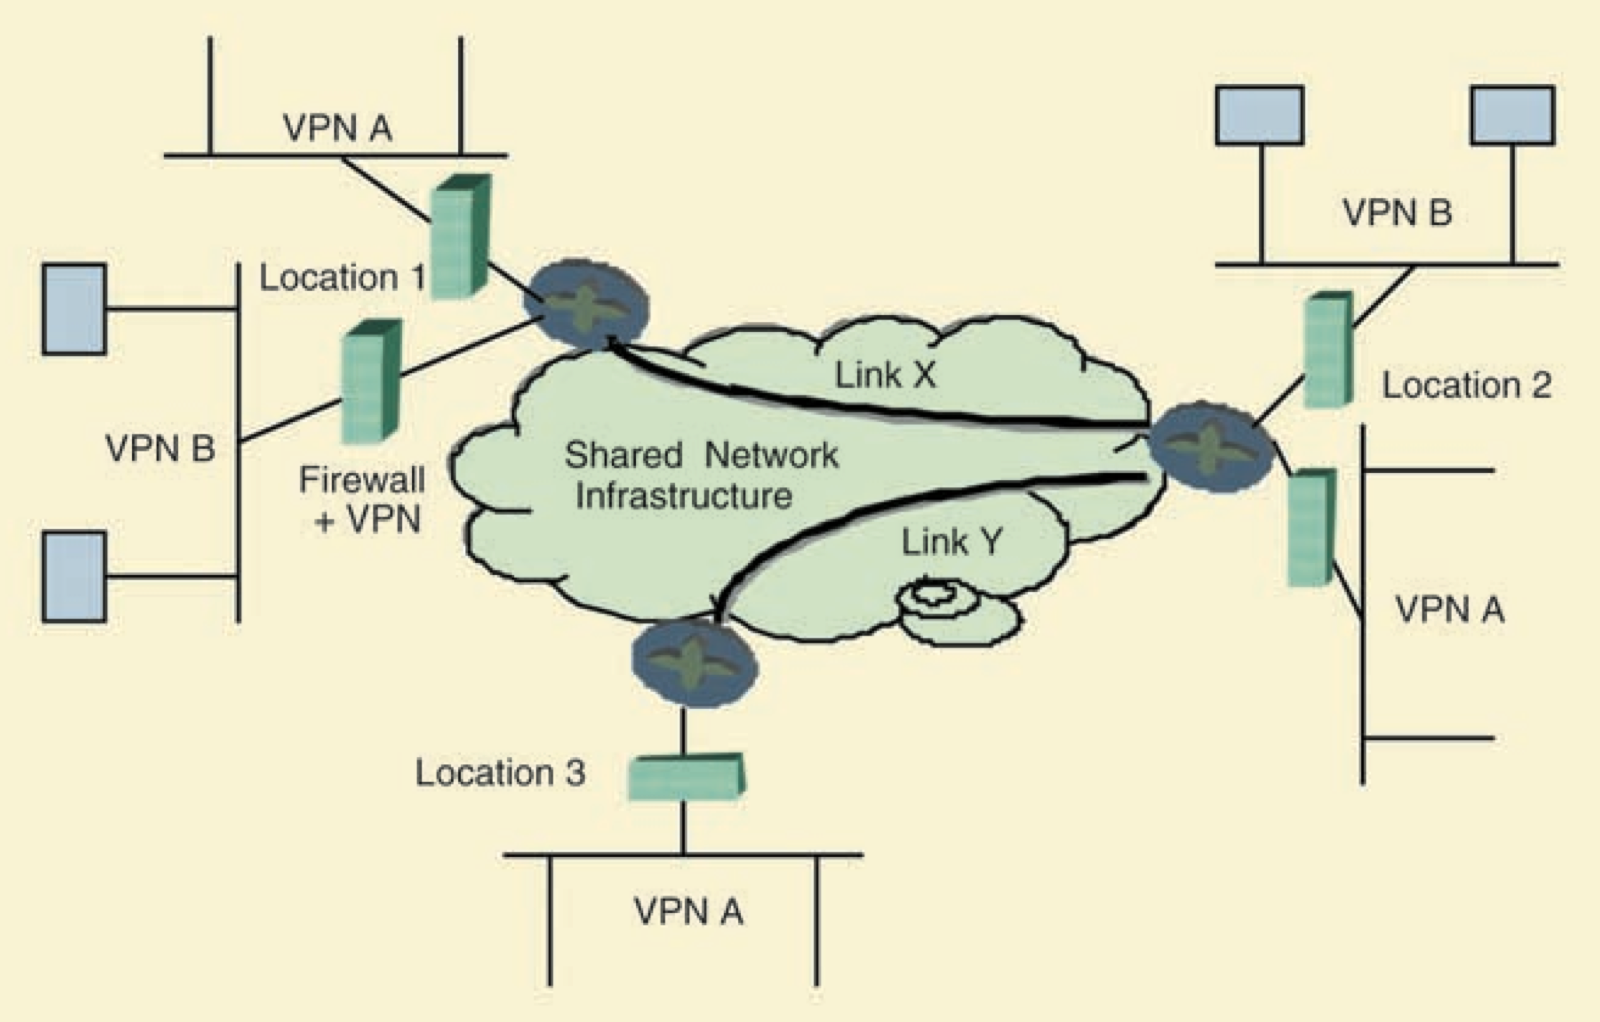
\includegraphics[width=5in]{../images/LAN-interconnect-VPN.png}%
\caption{LAN Interconnect VPN}
\label{fig:lan interconnect VPN}
\end{figure}
\bigskip

LAN Interconnect VPN services help to interconnect local area networks located at multiple geographic areas over the shared network infrastructure. Typically, this service is used to connect multiple geographic locations of a single company. Several small offices can be connected with their regional and main offices. This service provides a replacement for the expensive dedicated links. A simple LAN interconnect example is shown in the figure. VPN A has sites in geographic locations 1, 2, and 3, while VPN B has sites in geographic locations 1 and 2. Both vpns A and B are implemented on top of a shared network infrastructure. The advantage is the flexibility it offers \cite{venkateswaran2001virtual}.
Next, let us take a look at Dial-up VPN services. Please see Figure ~\ref{fig:Dial-up VPN}

\bigskip
\begin{figure}[hbt!]
\centering
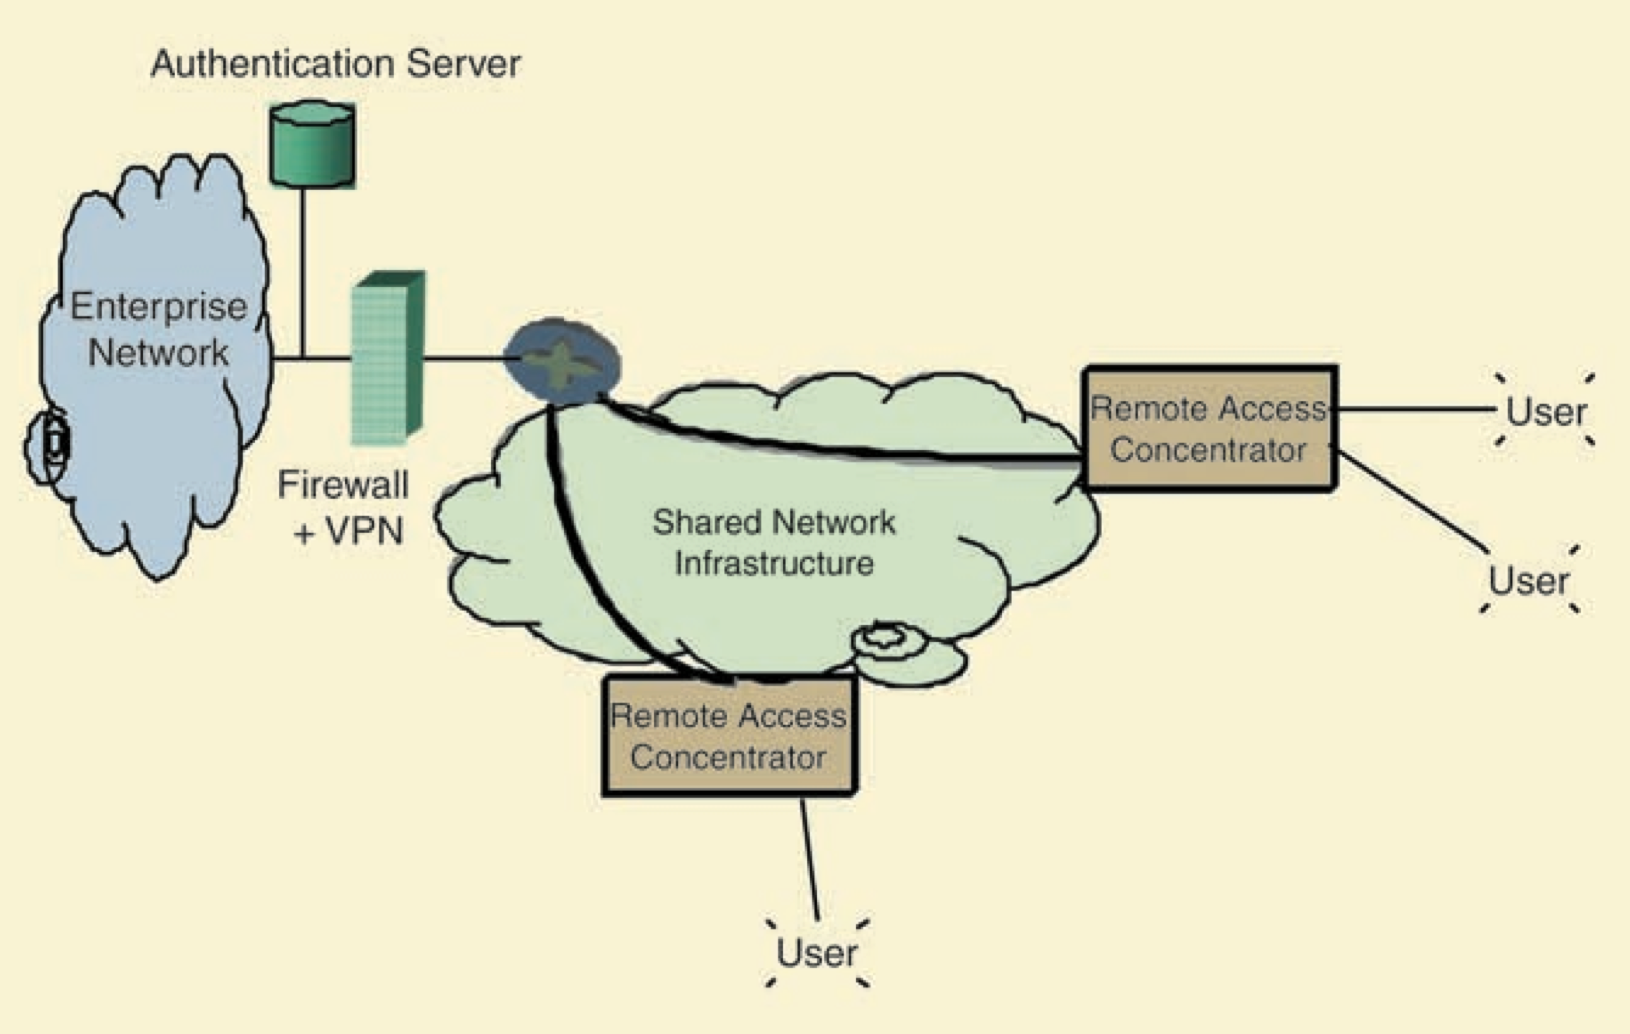
\includegraphics[width=5in]{../images/Dial-up-VPN.png}%
\caption{Dial-up VPN}
\label{fig:Dial-up VPN}
\end{figure}
\bigskip

From this diagram, we can see it is a bit different from the LAN VPN services. There is no VPN A or VPN B. Instead in this diagram the user is dialing into the closest remote access concentrator, which then connects to the shared network infrastructure and tries to make a clear connection to the VPN before it can have access to the server. Lastly, let us take a look at the Extranet VPN service. Please see Figure ~\ref{fig:Extranet VPN}

\bigskip
\begin{figure}[hbt!]
\centering
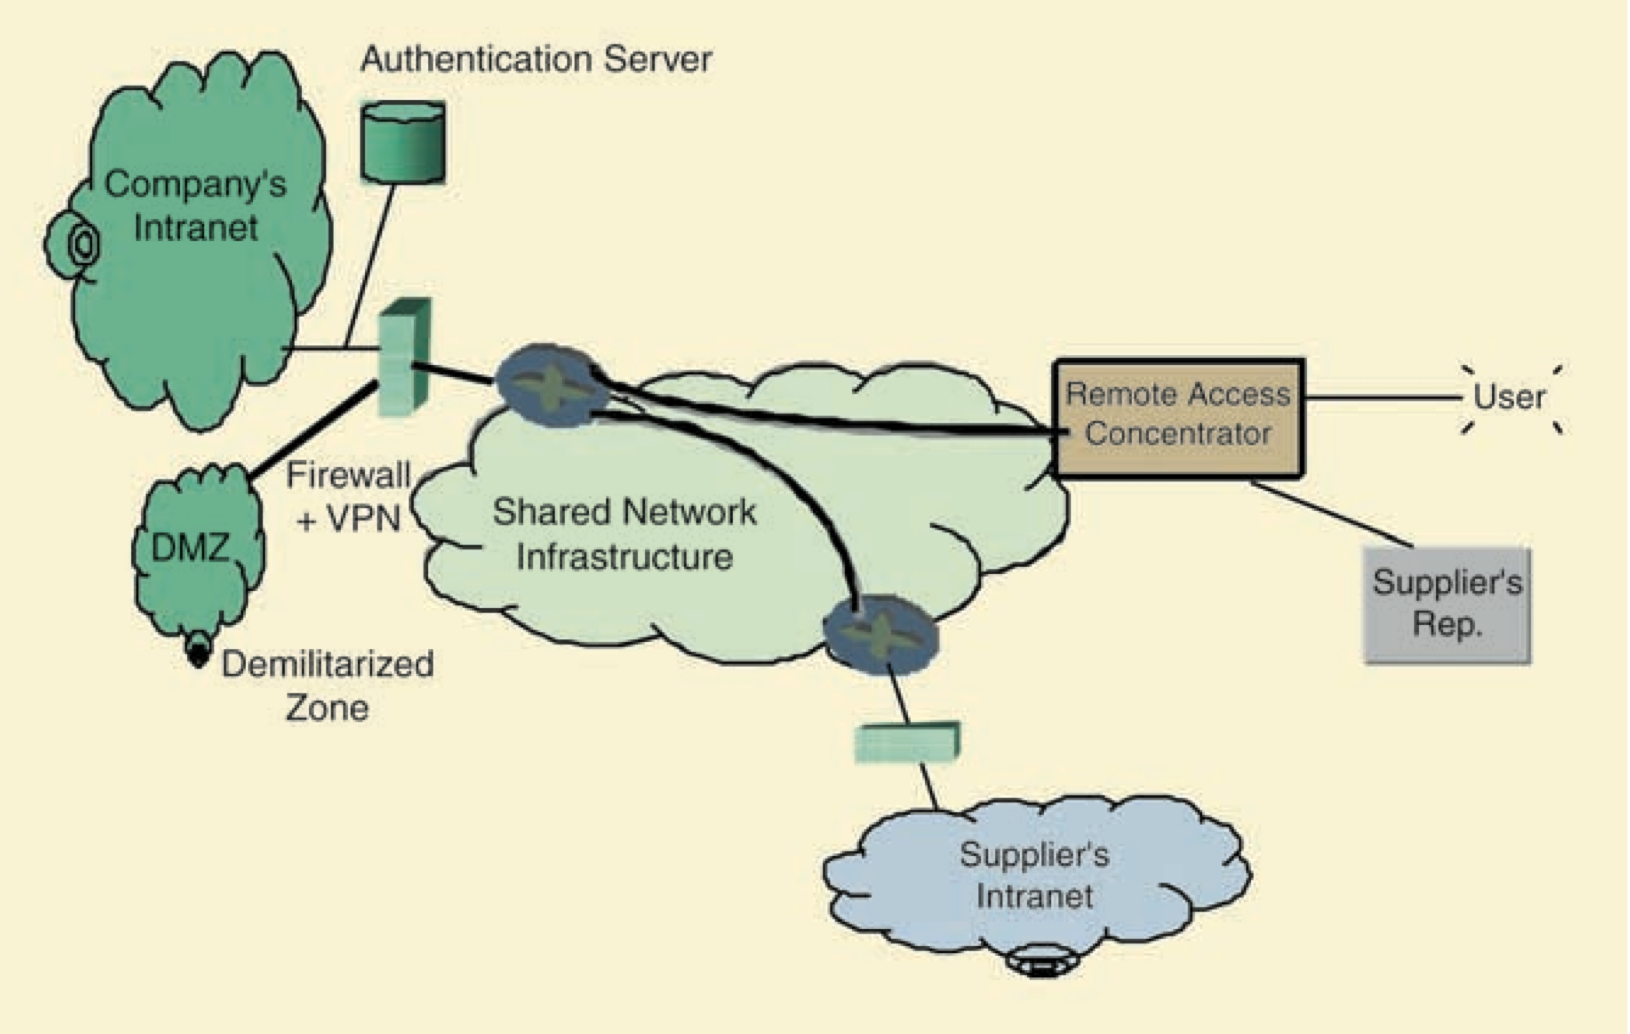
\includegraphics[width=5in]{../images/Extranet-VPN.png}%
\caption{Extranet VPN}
\label{fig:Extranet VPN}
\end{figure}
\bigskip

An Extranet VPN service shown in the figure combines the architecture of LAN Interconnect VPN services and dial-in VPN services. This infrastructure enables external vendors, suppliers, and customers to access specific areas of the company’s Intranet. The allowed specific area is denoted as the Demilitarized Zone (DMZ). When a packet is created by encapsulating and encrypting the original IP packet. The encryption keys and the algorithm parameters are negotiated and exchanged between the two VPN nodes using the Internet Key Exchange (IKE) protocols \cite{venkateswaran2001virtual}.


\section{Cloud Computing}
\label{sec:cloud computing}


Let us also try and understand more about cloud computing software. cloud computing software is something that we are all familiar with. Services such as Google, Amazon, and Microsoft all use cloud computing for their services. What exactly is it though? cloud computing is simply the availability of services in the cloud. The cloud computing idea emerges as a new computing paradigm that aims to provide reliable, customized, and QoS (quality of service) guaranteed dynamic computing environments for end-users \cite{wang2010cloud}.
Now that we know what cloud computing is, well what does it do? It allows infrastructures from the cloud to run their applications inside. There are three fundamental aspects of cloud computing. There is Hardware as a Service (Haas), Software as a service (Saas), and Data as a Service (Daas). Haas is when users buy IT hardware or in some cases even entire data centers using a subscription such as Amazon EC2. Saas is when the software or an application is hosted as a service. This eliminates the need for customers to download applications to their local computers. A modern example of this is Google Stadia's infrastructure or Spotify. Lastly, Daas is when data of any format can be accessed by users on a network. A big example of this is Google Docs \cite{wang2010cloud}.
All of these connect to the infrastructure (Iaas) which is then connected to the application. Please see Figure ~\ref{fig:Cloud Computing}


\bigskip
\begin{figure}[hbt!]
\centering
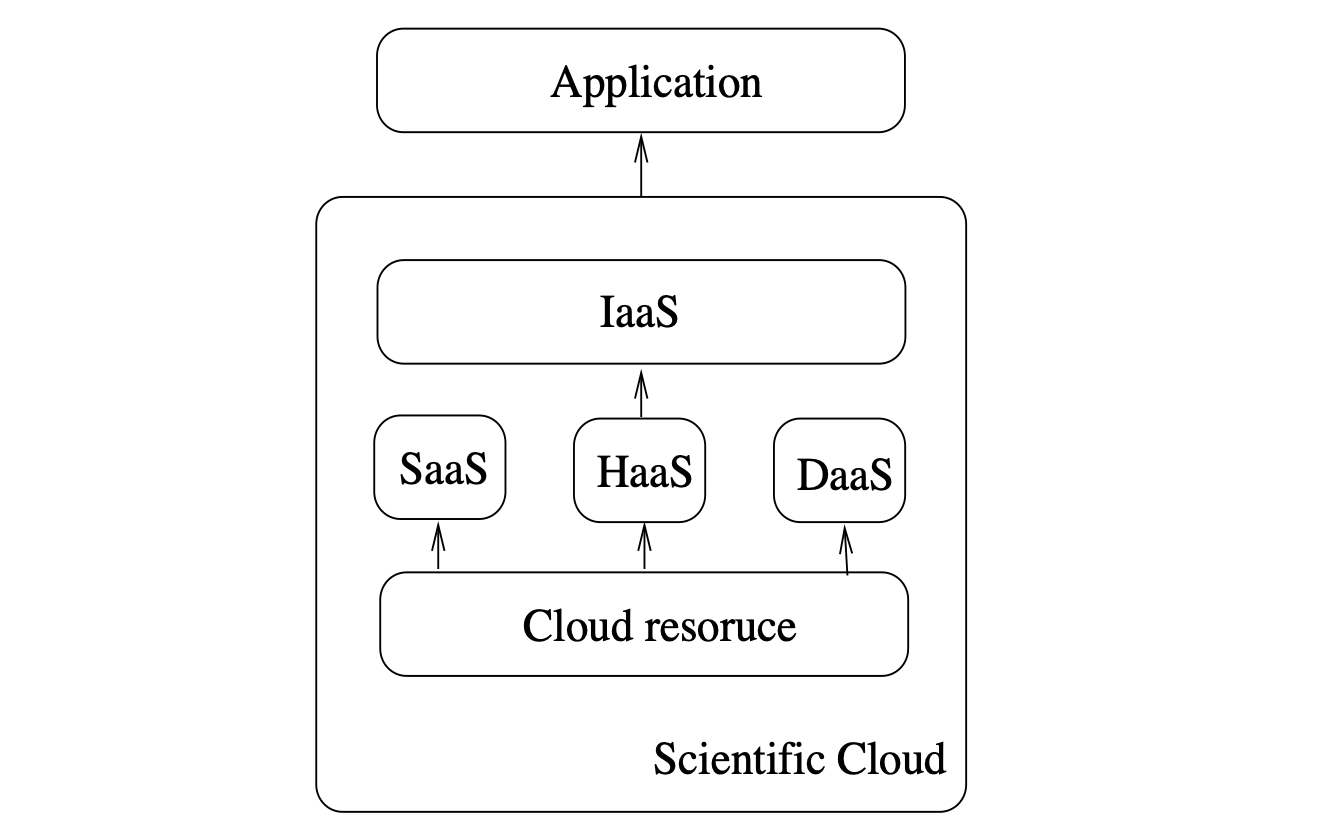
\includegraphics[width=5in]{../images/Cloud-Computing.png}%}
\caption{Cloud Computing}
\label{fig:Cloud Computing}
\end{figure}
\bigskip



\section{Goals of the Project}
\label{sec:goals}

The goal of this project is to show that vulnerabilities are a real problem in society today and this is something that we have to work towards fixing. Not only is the goal to show that these problems exist, but also to show that exploiting these problems is not as challenging as people make them seem to be. The result of someone being able to bypass login and infiltrate a database to extract valuable data is the result of sloppy code. When dealing with sensitive information like this, we cannot afford to let sloppy code be the downfall and have the possibility of somebody's sensitive information being stolen. There have been so many attacks that have been the result of sloppy code written in SQL and because of this, I have started to create my prototype that should help to mitigate against SQL injection attacks aimed at databases. My prototype simply just creates extra layers of protection that would make it much more difficult for someone to try and break into. With the use of VPN and cloud computing, it will add more layers of security because the VPN will hide your IP address from your ISP (Internet Service Provider) so people won't know where you will be logging in from and with the cloud computing structure, it will help keep your database from being accessed from unknown people or servers as you can create your server and manage who has access and who does not.


\section{Thesis Outline}
\label{sec:outline}

I carried out my proposed topic by performing a SQL injection attack on a web-based application with a database connected to it as this will allow me to get a clearer understanding of just the types of vulnerabilities that are prominent in web application and a database as it will show me just how dangerous a SQL injection attack can be. Performing a SQL injection attack showed me the security side of computer science which is very important since security is something that society as a whole benefits from. Since I did an attack on a web application, I had to make sure the web application that I performed the attack on didn't have any valuable data as I could have potentially ruined that data. After that, I had to start using SQL as a database and start using queries to be able to attack the web application and gain access to the data. For this proposed project, I attacked a web application using SQL injection with the hopes to concoct possible solutions to mitigate against vulnerabilities. I then started creating my prototype using cloud computing and VPN services as this will then help ensure more security as the database that is being accessed through the cloud won't be sitting on a dedicated server. The VPN will allow for more privacy for the user so their location services will not be revealed as a VPN changes your IP address and your online activity cannot be tracked. This will help protect the user so that nobody can track what they're doing or what web applications they are visiting. This then will help ensure the security of the user because if nobody can track your location or what web applications you might be visiting, then nobody will know that you are accessing a database through the cloud. With the knowledge I gained from being able to do a SQL injection attack, I will continue making my prototype that will help mitigate the risk of a hacker being able to use SQL injection to bypass a web application.
 % Introduction (first numbered chapter)

%\numberedchapter{Related Work}

\chapter{Related Work}
\label{ch:relatedwork}

\section{SQL Injection Techniques}
\label{sec:sql injection techniques}
The way I conducted my study and performed my injection attack was by first having to fully understand what it was I was supposed to do, the best way to do that was to study works and attacks that had already been done that are related to mine. The first article that I ran into is "  Vulnerability assessment \& penetration testing as a cyber defense technology." This article relates to my work because it discusses and aims at penetration testing. The article first goes on to talk about exactly what a vulnerability is. A vulnerability is a weakness in the application which can be an implementation bug or a design flaw that allows an attacker to cause harm to the user of the application and get extra privilege \cite{goel2015vulnerability}.
The article then goes on to talk about vulnerabilities and penetration testing. The main focus of this article is to explain that penetration testing and vulnerability assessments are good techniques to use as a way of cyber defense technology. After the paper has discussed the terminology of what it is they are doing, the paper then goes on to talk about the various techniques that can be used as well as tools that can be used. The paper then concludes by stating that the whole goal of the paper was to inform people about penetration testing and it is used that it has as a cyber defense system. It states that using these tools will allow researchers to develop stronger security solutions.

This study "Advanced SQL injection in SQL server applications" gives it is research on SQL injection in applications. The abstract of this document, explains what the article aims to do. The article talks about the most common 'SQL injection' technique as it applies to the popular Microsoft Internet Information Server. It discusses the various ways that SQL can be injected into the application and addresses some of the issues that are related to this kind of attack \cite{anley2002advanced}.
The introduction of the article, explains and talks about what SQL is and how it relates to databases. SQL injection occurs when an attacker can insert a series of SQL statements into a 'query' by manipulating data input into an application. A typical SQL statement looks like this:
'select id, forename, surname from authors'. In this situation, an attacker can simply append SQL statements at the end of the numeric input. In other SQL dialects, various delimiters are used; in the Microsoft Jet DBMS engine, for example, dates can be delimited with the pound character. The article gives an example code of possible situations and what you might see while you might attempt to perform a SQL injection attack. After the article goes on to talk about possible code you might see with some examples, it then goes into very explicit detail about databases and servers. SQL Server provides a mechanism to allow servers to be 'linked' - that is, to allow a query on one database server to manipulate data on another. The concluding remark about this article simply talks about the importance of why you need to 'lock down the SQL server and gives a list on how to build a SQL server. Overall, this article relates to my work as the goal of this project was to perform a SQL injection attack and this article gives numerous examples and scenarios of possible things that could've happened to me. This article goes into a lot of detail about the steps that you would need to take as well as giving you example query statements of what you might type.



\section{Vulnerability Tools}
\label{sec:Vulnerability Tools}

There are many tools used to test vulnerabilities and this article "Testing and comparing web vulnerability scanning tools for SQL injection and XSS attacks" goes into depth explaining how they can be compared against attacks. This article first talks about how web applications are usually made with a time constraint and because of that, they are usually vulnerable to attacks because of a lack of security measures. The whole point of this article is to discuss the available scanning tools that are out there for SQL injection so that one may not necessarily worry too much about that. Web applications are extremely popular today. Nearly all information systems and business applications (e-commerce, banking, transportation, webmail, blogs, etc) are now built as web-based database applications. They are so exposed to attacks that any existing security vulnerability will most probably be uncovered and exploited, which may have a highly negative impact on users. Automatic web vulnerability scanners are often used by web application developers and system administrators to test web applications against vulnerabilities. Therefore, trusting the results of web vulnerability scanners is essential \cite{fonseca2007testing}.
The article then goes on to talk about security measures and the detection of vulnerabilities within web applications. There are two main approaches to test web applications for vulnerabilities: “white box” and “black box”. To simply explain what each of these techniques is, white box is essentially a technique used when the attacker has an understanding of the network that they are trying to get into whereas black box is the opposite, the attacker doesn't have much knowledge when it comes to the knowledge of the network they are trying to get into. This article had a case study that they did. For the evaluation experiments, we used LAMP (Linux, Apache, Mysql, and PHP) web applications. The server runs Linux and the web server is Apache. This server hosts a PHP-developed web application using a Mysql database. The authors had used three commercial web application vulnerability scanners, that we named Scanner 1, Scanner 2, and Scanner 3. They decided to keep the brand and the versions of the web vulnerability scanners anonymous to assure neutrality and because commercial licenses do not allow in general the publication of tool evaluation results. When conducting the test, they put a table of their finding and found that SQL injection had a higher percentage in all 3 scanner techniques. In the conclusion of this article, they talk about their findings and how to use more web applications so that they can understand the relationship between software faults and vulnerabilities. This work relates to mine because as someone interested in SQL injection I also understand how it may affect a web application and which types of attacks might work.



\section{Intrusion}
\label{sec:Intrustion}

As we have seen there are lots of studies out there about SQL injection and this article "Application Layer Intrusion Detection for SQL Injection" talks about how it can be used with intrusion detection. This article first starts by talking about the motivation of their work. Web applications are becoming increasingly commonplace and accessible. Often the developers of these programs are focused on getting a working application under time pressure and may not implement the best security practices \cite{rietta2006application}.
It then goes on to talk about SQL injection and the different techniques that are associated with that type of injection attack. SQL injection is a technique often used to exploit database systems through vulnerable web applications. The technique allows the attacker to not only steal the entire contents of relational databases but also, in many cases, to make arbitrary changes to both the database schema and the contents. This article aims to examine the threat from SQL injection attacks, the reasons traditional database access control is not sufficient to stop them, and some of the techniques used to detect them. Moreover, it proposes a model for an anomalous SQL detector that observes the database from the perspective of the database server itself. In the conclusion of this article, it talks about possible plans and what it wants to do. In the conclusion, they state that they want to research additional measures to take that could mitigate SQL injection attack risks. This work relates to mine because just like I said earlier, to fully be able to understand what SQL injection is and how it affects other applications, I believe it was also essential for me to understand what measures are taken that used to defer SQL injection attacks.

\section{SQL and Web Applications}
\label{sec:sql & web applications}
In this article "SQL injection." The first thing this article does is ask you "Are your web applications vulnerable?" After that in the Introduction, it gives a little background on web applications and SQL injection. SQL injection is a technique for exploiting web applications that use client-supplied data in SQL queries but without first stripping potentially harmful characters. Despite being remarkably simple to protect against, there is an astonishing number of production systems connected to the Internet that are vulnerable to this type of attack \cite{spett2002sql}.
The objective of this article is to focus the professional security community on the techniques that can be used to take advantage of a web application that is vulnerable to SQL injection and to make clear the correct mechanisms that should be put in place to protect against SQL injection and input validation problems in general. Just like an article, I discussed earlier, this article goes in-depth about how you might perform an injection attack, the types of things you might see, and then how you may fix these security errors. This article relates to my work simply because it shows how one might perform a SQL injection attack which was very helpful to me.


\section{Evading SQL injection}
\label{sec:Evading SQL injection}

Over the numerous articles out there, this article "SQL injection signatures evasion" explains how to evade SQL injections. In this paper, the introduction first starts by looking at a theoretical hacker and gives a theoretical scenario. After that, the article then goes into talking about how this theoretical person may hack a system and informs us about the possible solutions the developers of that system could've taken to ensure that the hack couldn't take place or at least be a lot more difficult to take place. In recent years, Web application security has become a focal center for security experts. Application attacks are constantly on the rise, posing new risks for the organization. One of the most dangerous and most common attack techniques is SQL Injection, which usually allows the hacker to obtain full access to the organization's Database \cite{maor2004sql}.
The paper further demonstrates why these techniques are just the tip of the iceberg of different evasion techniques, due to the richness of the SQL language. Eventually, the conclusion that the research leads to is that protecting against SQL Injection using only signatures is simply not practical. This article relates to my work because like most of the other articles I have mentioned, it discusses theoretically how a system might be hacked and how there could be some measures taken to ensure that did not happen.

Several studies talk about SQL injection and this article "Defeating SQL injection" specifically talks about guarding against SQL injections. Just like the first article I talked about, "Vulnerability assessment \& penetration testing as a cyber defense technology", this article talks about SQL injection as a means of defending against it. The best strategy for combating SQL injection, which has emerged as the most widespread website security risk, calls for integrating defensive coding practices with both vulnerability detection and runtime attack prevention methods \cite{shar2012defeating}.
This article first talks about the SQL query language and it is common uses. Structured query language is a code injection technique commonly used to attack websites in which the attacker inserts SQL characters or keywords into a SQL statement via unrestricted user input parameters to change the intended query's logic. After the article talks about the SQL query language, it then goes into some coding practices and talks about some of the types of databases you can use that will access a server and how developers make mistakes that often lead to vulnerabilities. SQL is the standard language for accessing database servers, including MySQL, Oracle, and SQL Server. Web programming languages such as Java, ASP.NET, and PHP provide various methods for constructing and executing SQL statements, but, due to a lack of training and development experience, application developers often misuse these methods, resulting in SQL injection vulnerabilities (SQLIVs). The article then goes on to talk about some examples of vulnerabilities that a developer might make. An example of a mistake would be "Absence or misuse of delimiters in query strings". When constructing a query string with inputs, a programmer must use proper delimiters to indicate the input’s data type. The absence or misuse of delimiters could enable SQL injection even in the presence of thorough input validation, escaping, and type checking. After giving an example of a possible vulnerability, the article would then give some example code of what someone might see. This article aims to shed light on possible vulnerabilities that developers make so that they won't make this mistake, thus making it harder for someone to perform a SQL injection attack on their code. Where this article relates to my work is mainly in the conclusion section. In the conclusion, this author goes on to talk about how these defenses against SQL injection have both their strengths and their weaknesses. This was good for me because then I was able to get a broader understanding of vulnerabilities and gave me some ideas about how I might do my attack.

\section{SQL Detection}
\label{sec:SQL Detection}


Many studies have been on SQL injection and this article "Detecting SQL injection vulnerabilities in web services" explains how it affects websites. This article first talks about web services and their components and how they are becoming a strategic component in a wide range of organizations. Also, web services are extremely exposed to attacks. Any existing vulnerability will most probably be uncovered/exploited \cite{antunes2009detecting}.
The article aims to show that the approach that they decide to take is a better one than just using a traditional approach that scanner tools use and they provide their results and their findings in a table. In the conclusion of this article, they explain why the tool that they built is better. Our tool was able to detect vulnerabilities that were not detected by the commercial scanners. This work relates to my research because when doing a SQL injection attack, I don't know the type of security the web application is using so this article helps explain that when performing an attack you cannot assume anything about security.

\section{Cloud Infrastructure}
\label{sec:cloud infrastruture}
With the start of the implementation of my prototype, I had to use a type of technology called cloud computing. In "Secure User Data in Cloud Computing Using Encryption Algorithms" cloud computing is transforming information technology. As information and processes are migrating to the cloud, it is transforming not only where computing is done, but also fundamentally, how it is done \cite{arora2013secure}.
This piece explains how important and fundamental cloud computing is when it comes to solving modern-day problems in academics and a working environment. The article explains how new things such as data security and data ownership have made it difficult for normal approaches. Where the article is important to my work is when it starts talking about security issues and challenges in cloud computing. A big problem that this article talks about is the integrity of the data meaning that the data would not be changed unless authorized. The proposed plan that this article talks about is creating an algorithm that eliminates the concerns regarding data loss, and privacy while accessing the web. This article relates to my work because I am implementing a tool using a cloud computing platform to get rid of some of the data and privacy issues that plague information technology processes.

Just as the previous article mentions, there are lots of security issues that cloud computing tries to address. In "Addressing cloud computing security issues" talks about some of those issues. The recent emergence of cloud computing has drastically altered everyone’s perception of infrastructure architectures, software delivery, and development models \cite{zissis2012addressing}.
This paper sheds light on something that is not new in the computer science world, but it is something that I haven't quite seen talked about. When this article addresses the idea of security, it then talks about trust. For the concept and system to work as expected, there must be mutual trust going on. This overall helps with credibility and reliability. The next important concept that this article talks about that also pertains to me is security identification of threats. The information system must identify threats so proper countermeasures can be taken. This concept and idea relate to my work because I have to make sure I am identifying the important security issue(s) surrounding my web application and database so then I can create a prototype using a cloud computing service and eliminate those threats.

\section{VPN services}
\label{sec:VPN services}
When I started implementing my prototype, I needed to use a VPN. This will help change the IP address of the user which in turn will help with better security. This approach is also very important when accessing public and private cloud computing services. In "An automated implementation of hybrid cloud for performance evaluation of distributed database" talks about the idea of hybrid cloud. A Hybrid cloud is an integration of resources between private and public clouds. It enables users to horizontally scale their on-premises infrastructure up to public clouds to improve performance and cut up-front investment costs. This model of application deployment is called cloud bursting that allows data-intensive applications, especially distributed database systems to have the benefit of both private and public clouds \cite{mansouri2020automated}.
According to the article, IT businesses have a large desire to exploit hybrid cloud services. This brings a potential capability to implement a consistent hybrid cloud through VPN. This work is related to my project because I too plan on using a VPN to help with privacy issues when connecting to a database through the cloud.

With time permitting and my prototype shedding possible security solutions, I needed to use a VPN. In "Design of Border Security Defense System for VPN Network in Power Enterprises" explains the importance of using a VPN. This article talks specifically about using a VPN in power enterprises but the concept is very similar to my work. To ensure the safe and stable operation of the power system, the VPN network border security defense system of power enterprises is designed. The hardware of the system is planned and designed, including cooperative intrusion detection, security audit, cooperative camouflage, collaborative firewall, disaster recovery, and electronic forensics \cite{wenzhen2020design}.
Just like my possible solution with my project. A VPN is very important when it comes to doing work online. It allows for privacy and as the article put it, "camouflage".

Why are VPNs so popular today? well in "Virtual Private Networks'' explains the explicit uses of a VPN and why it is so popular today. Let's first start with what a VPN is. A VPN is a Virtual Private network \cite{venkateswaran2001virtual}.
Well, what does that look like? Let's first characterize a VPN. It is a private network that supports a closed community of authorized users, allowing them to access various network-related services and resources \cite{venkateswaran2001virtual}.
Now let us answer the first question that we had asked. Why are VPNs so popular today? Traditional private networks facilitate connectivity among various network entities through a set of links, comprising the dedicated circuit. VPN services enable remote access to the Intranet at a significantly lower cost, thus enabling support for a mobile workforce. Additionally, the VPN architecture supports a reliable authentication mechanism to provide easy access to the Intranet from anywhere using any available access media including analog modems, ISDN, cable modems, DSL, and wireless. There are multiple types of VPN services. The three primary sources of VPNs are Local Area Networks, Dial-up VPN, and Extranet VPN services. LAN Interconnect VPN services help to interconnect local area networks located at multiple geographic areas over the shared network infrastructure. Typically, this service is used to connect multiple geographic locations of a single company. The Dial-up VPN service supports mobile and telecommuting employees in accessing the company’s Intranet from remote locations. An extranet VPN service combines the architecture of LAN Interconnect VPN services and dial-in VPN services. This infrastructure enables external vendors, suppliers, and customers to access specific areas of the company’s Intranet.
A big aspect of the prototype that I plan on implementing uses cloud computing. According to "Cloud Computing: A Perspective Study'' A computing Cloud is a set of network-enabled services, providing scalable, QoS guaranteed, normally personalized, inexpensive computing infrastructures on demand, which could be accessed in a simple and pervasive way \cite{wang2010cloud}. There are three fundamental aspects of the cloud computing platform. There is Hardware as a Service (Haas), Software as a service (Saas), and Data as a Service(Daas). With Haas, IT automation, and usage metering and pricing, users could buy IT hardware, or even an entire data center, as a pay-as-you-go subscription service. The Haas is flexible, scalable, and manageable to meet your needs \cite{wang2010cloud}. With Saas, Software or an application is hosted as a service and provided to customers across the Internet. This mode eliminates the need to install and run the application on the customer’s local computers. SaaS, therefore, alleviates the customer’s burden of software maintenance and reduces the expense of software purchases by on-demand pricing. An early example of the SaaS is the Application Service Provider. Lastly, with Daas, Data in various formats and from multiple sources could be accessed via services by users on the network. Users could, for example, manipulate the remote data and operate on a local disk or semantically access the data on the Internet. DaaS could also be found at some popular IT services such as Google Docs \cite{wang2010cloud}.




%\numberedchapter{Method Of Approach}

\definecolor{dkgreen}{rgb}{0,0.6,0}
\definecolor{gray}{rgb}{0.5,0.5,0.5}
\definecolor{mauve}{rgb}{0.58,0,0.82}

\lstset{frame=tb,
  language=Java,
  aboveskip=3mm,
  belowskip=3mm,
  showstringspaces=false,
  columns=flexible,
  basicstyle={\small\ttfamily},
  numbers=none,
  numberstyle=\tiny\color{gray},
  keywordstyle=\color{blue},
  commentstyle=\color{dkgreen},
  stringstyle=\color{mauve},
  breaklines=true,
  breakatwhitespace=true,
  tabsize=3
}




\chapter{Method of Approach}
\label{ch:method}

\section{Design Overview}
\label{sec:design overview}


The first step to completing the proposed research and to also make sure that everything
would have been accurately accounted for was by first planning out what exactly was necessary
for us to do. Since the topic of this project was to do a SQL injection attack, something that needed to be thought about was what was going to be attacked. SQL injection attacks are typically done against
web-based applications so the plan was to target a web application to do the attack on. After
figuring out that the attack was going to happen to a web application the next step was to think of a specific web application that we could target to properly learn but also
keep in mind that one cannot just perform an attack on any regular web application as that would
not be an ethical thing to do. After talking with my readers, the best option that
we had decided was to create a "dummy" web application as this would allow
me to be able to not only perform a SQL injection but to also have the peace of
mind knowing that if the attack did indeed accidentally made a change to the web application that
there would be harm done to anybody else's work in the process. The framework that was chosen was flask for the creation of this web application. Although there are other options out there
such as Django and streamlit, flask was mostly familiar to me with its design
and also the fact that it uses python as its coding language. Flask also allows for the ability to format the web application and make it look the way we want it to look. The topic
that was chosen for this project isn't common knowledge for everyone so thinking about how others
could navigate when they are on the web application was an important thing to think about. When making the web application it was important to make
the design and layout of the site not only user-friendly but also make sure that
included somewhere on the site a place where the SQL injection could happen. We had chosen
to use a simple layout with not many web pages as this should help people easily
navigate and also understand and follow along with everything that we had decided
to do. We created the site to act as a mock-up for what a banking web application would look like, just to
try and reel in the user and make the illusion that they are actually on a banking
web application with the idea that they are going to inject SQL code to by-pass the
security and gain access to sensitive data. If the user can be engaged to
the fact that they are actually about to try and bypass a login screen by gain access to sensitive information then this project should resonate with them. After all,
everyone who has some sort of money has a bank account, so if we can portray to the user that bypassing login is not quite as difficult as it seems, then
one can believe people will start taking their privacy a lot more seriously. After making
sure we had done everything that we wanted to do and the web application was created, we had
then done the SQL injection attack.


\section{Libraries}
\label{sec:libraries}


When creating the web application using flask, we had to use certain libraries to make sure that we had everything that we needed to ensure that the web application ran properly. we needed to choose ones that would allow me to integrate python with the web application that we needed to create. The first major library that we needed to use in the main program file was, of course, flask. Importing this library would allow me to use the Flask framework and pick a nice template that we could use as a starting point for the web application. The next main library that we needed to use was SQLAlchemy. This library will allow me to create and execute SQL code in the program without having to write SQL statements. For the app file, we needed to import more libraries from flask, but we needed to import specific ones. The ones that we needed to import were render-template, redirect, URL-for, request, and g as well as SQLite3. These specific libraries will allow me first, render the template that we had chosen from flask. Then the redirect library will allow me to redirect the user to a different page if the required requirements were met. The "URL-for" will allow me to redirect the user to a different page using its URL. Request will allow me to ask the user for some type of input. Lastly, g will allow me to connect the database to the web application and have access to it. Using these libraries allowed me to integrate everything that we needed to not only create the flask web application with python but also connect the database to the web application so that the data can be displayed on the web application. Please see Figure ~\ref{fig:web app home page} the web applications interface.


\bigskip
\bigskip
\begin{lstlisting}
from flask import Flask, render_template, redirect, url_for, request, g
import sqlite3
app = Flask(__name__)
app.database = "data.db"
\end{lstlisting}
\bigskip
\bigskip



\bigskip
\bigskip
\begin{figure}[hbt!]
\centering
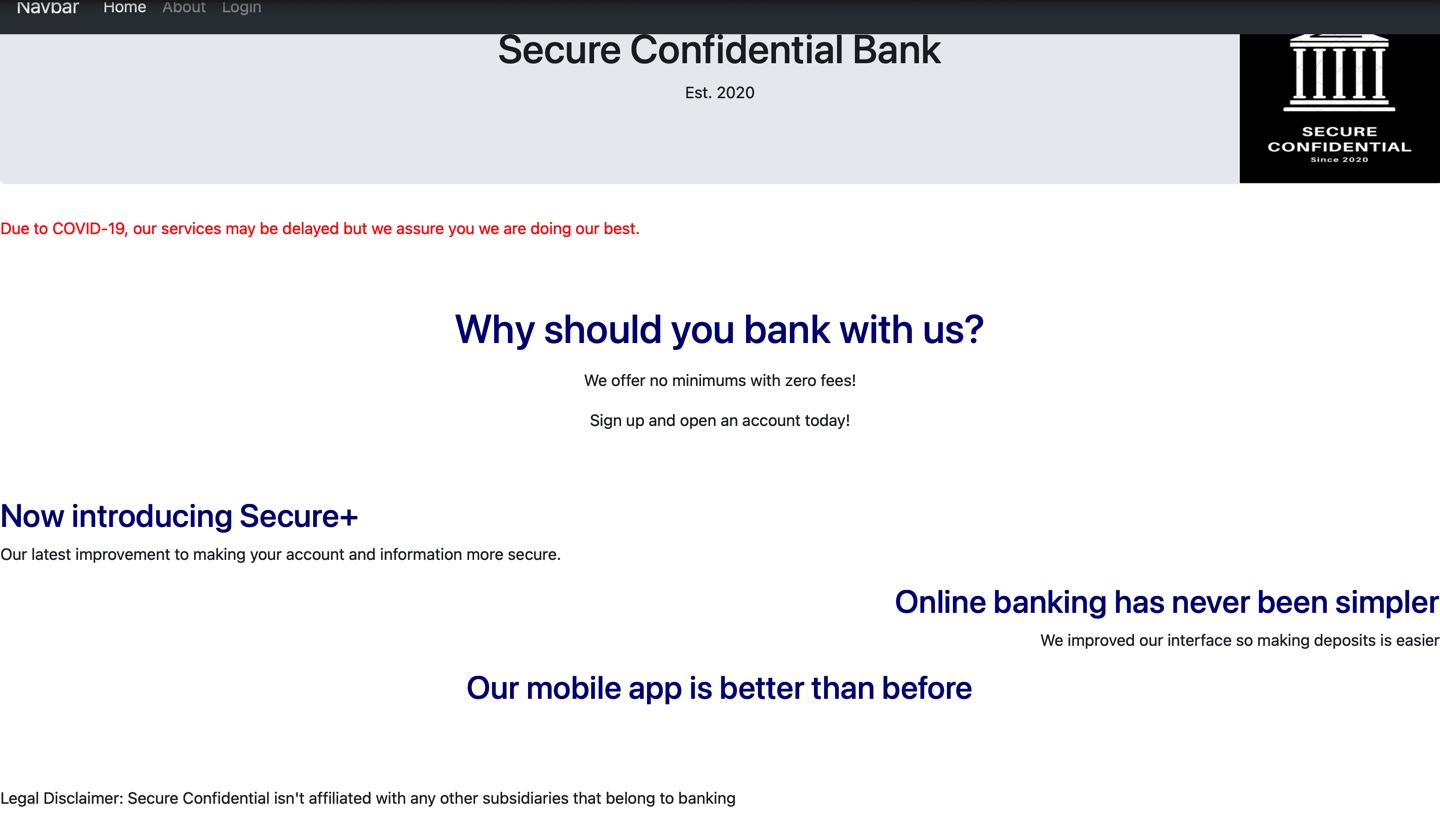
\includegraphics[width=5in]{../images/website.png}%
\caption{Web App Home Page}
\label{fig:web app home page}
\end{figure}

\bigskip
\bigskip


\section{Python Functions}
\label{sec:python functions}

While creating the program in python to create the web application and connect the database, we needed some functions that we could do a few things. First, we needed to create some functions that would allow me to route the links to certain pages on the web application. For example, if we had an about page on the web application, we needed to route the actual about button on the web application to the about page on the web application. The same goes for a home page and the login page. When we talk about the login page though, things can get a little tricky. Once we had routed the login button to the login page, we also needed to route the "success" page that displays all the data within the database but only if one could successfully login. With that being said, we also needed to return the "Invalid" statement if the credentials that one had entered were incorrect. This is where the idea of conditional logic comes in. Conditional logic is simply a set of rules one can place that causes ones process to be changed based on the given input. There are a few different types of conditional logic but here we are just going to focus on one type. The type of conditional logic that we are going to focus on is IF statements. An IF statement simply reads, IF - "this sort of action takes place" then produces this output. What we utilized with the IF statement as well was an else condition. It follows the same pattern as an IF statement. IF - "this sort of action takes place" then produce this output, ELSE - produce this output. You can get the idea of how one can play around with this in programming and that's exactly what we did. we created this thing called a nested loop which allows me to put multiple conditional logic statements within each other. This will allow me to be able to route the "success" page, and the "Invalid" statement if certain conditions were met. All in one function.

\begin{lstlisting}
if username is None:
            error = 'Invalid Credentials. Please try again'
            return render_template('log.html', error=error)
        else:
            return redirect(url_for('hello'))
    else:
        return render_template('log.html', error=error)
\end{lstlisting}

\bigskip
\bigskip

\begin{lstlisting}
@app.route('/')
def home():
    return render_template('home.html')
\end{lstlisting}


\section{HTML and Web Applications}
\label{sec:html and web applications}

When we had created the "dummy" web application and performed the actual SQL injection attack,
we needed to utilize some coding languages as well as databases if we were to properly
and effectively conduct the injection attack. The first coding language
that we had to utilize is HTML. This was imperative because this is the
language that we used while creating the "dummy" web application. HTML simply
stands for hyper-text markup language and this is a web-based language commonly
used when creating a web application. we had decided to use HTML because of its easy-to-understand
language as well as its simplistic syntax. HTML is widely known and used today. Below
is some code from the web application that is in HTML. As one can see, this simply is displaying
text from the about page on the web application.

\bigskip
\bigskip
\begin{lstlisting}



  <div class="jumbotron text-center">
    <h1>About us</h1>
    <p>We are committed to keeping your information secure.</p>
    <image src="{{ url_for('static', filename='images/thesecure.png')}}" width="200" height="180" style="position:absolute; right:-41px; top:43px">
  </div>
    <body>
      <h1><center>Privacy is our top priority</center></h1>
      <p>Here at secure confidential, we pride ourselves on giving our customers world class security to ensure them with the peace of mind knowing that their information is safe and secure. After all, everyone is entitled to have privacy. We can also safely say that we have had zero security issues thus far. Putting your information in someone elses hands is scary, that is why we make it easy to do so. Consider banking with us as we promise your account information is safe and secure.</p>
      <br><br>
      <h2 style="color:navy"><center>Consider these practices when it comes to managing your security</center></h2><br>
      <h3 style="color:red"><center>Regularly change your password</center></h3>
      <p><center>Regularly changing your password will make it harder for others to try and steal your information</center></p><br>
      <h3 style="color:red"><center> Never write down any of your information</center></h3>
      <p><center>Writing down your information could lead to theft</center></p><br>
      <h3 style="color:red"><center> Set up your alerts</center></h3>
      <p><center>Having your alerts on your phone will always allow you to get a notification of transactions in your account in real time</center></p><br>

    </body>




\end{lstlisting}
\bigskip
\bigskip

\section{SQL and Databases}
\label{sec:sql and databases}


The next and important database language that we had to use was SQL. This should not
be a surprise as the title of the thesis is "Assessing vulnerabilities using
SQL injection". We chose SQL because there are a lot of known security issues associated
with SQL and web-based applications. SQL injection is a very common and widely known
technique to attack databases so we wanted to not only see how this was possible
but also figure out why this might be the case and if there are any ways to fix
or mitigate this type of vulnerability. The way we had set up the database though, we had
tried to continue to follow the pattern and idea of how a bank might set up their database.
For simplicity, we had created one database with multiple tables. We can imagine though,
on a much larger scale, there would probably be multiple databases which would make this
process a little more difficult but still, the concept would be the same. The three
tables that we had decided to use were Customers, Managers, and Employees. The way
that we created the database was pretty simple, we decided to use a GUI (graphical user
interface) to set up the columns, rows, and tables in the database because it is a lot
simpler to do it that way, but traditionally, lots of people decide to use the command-line interface for this type of approach. Either way, each option is viable. Please see Figure ~\ref{fig:tables in terminal}.

\bigskip
\bigskip
\begin{figure}[hbt!]
\centering
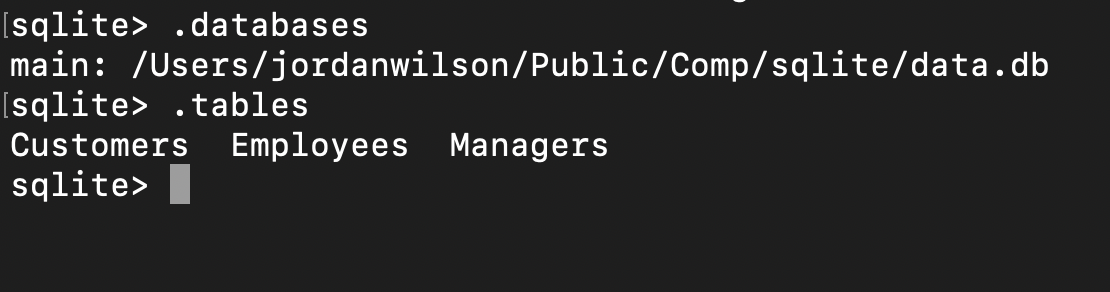
\includegraphics[width=5in]{../images/sql-terminal.png}%
\caption{Tables in terminal}
\label{fig:tables in terminal}
\end{figure}
\bigskip
\bigskip



The next big and important thing that we had to do was to populate the database. We needed
to do this to get all of the data that is not only going to be in
the database but also be displayed on the web application. The approach for doing this was to
simply import a CSV document with lots of fake data. We needed to do this because first,
we obviously could not use real data and second, we wanted a lot of fake data to represent
people and it would take a long time to manually insert all of that data into the
database, not to mention we would have to come up with all of the fake data ourselves, so
we just opted to have a web application generate a lot of fake data and then we were able to import
it. When generating the fake data though, we had to keep in mind the type of
information that we wanted to be displayed in the database. A big proponent of the
project is also the ethics associated with the data that is inside of databases so
we had chosen a bunch of variables that had to show that all of these people have very
private and sensitive information. The types of rows and columns that we had decided to
use were firstname, lastname, age, street, city, state, zip, salary, eye color, dob, religion,
political affiliation, relationship status, and ethnicity. As one can see, a lot of
these factors should not matter to set up a bank account. We had done this to show
that a lot of companies are asking us more information than they need for people
to set up an account with them. This also poses a security issue because if that specific
company has their database breached (which we show in this project) then a lot of people's
sensitive information is shown. Information that does not need to be in a database by some
company. Please see Figure ~\ref{fig:table info}.

\bigskip
\bigskip
\begin{figure}[hbt!]
\centering
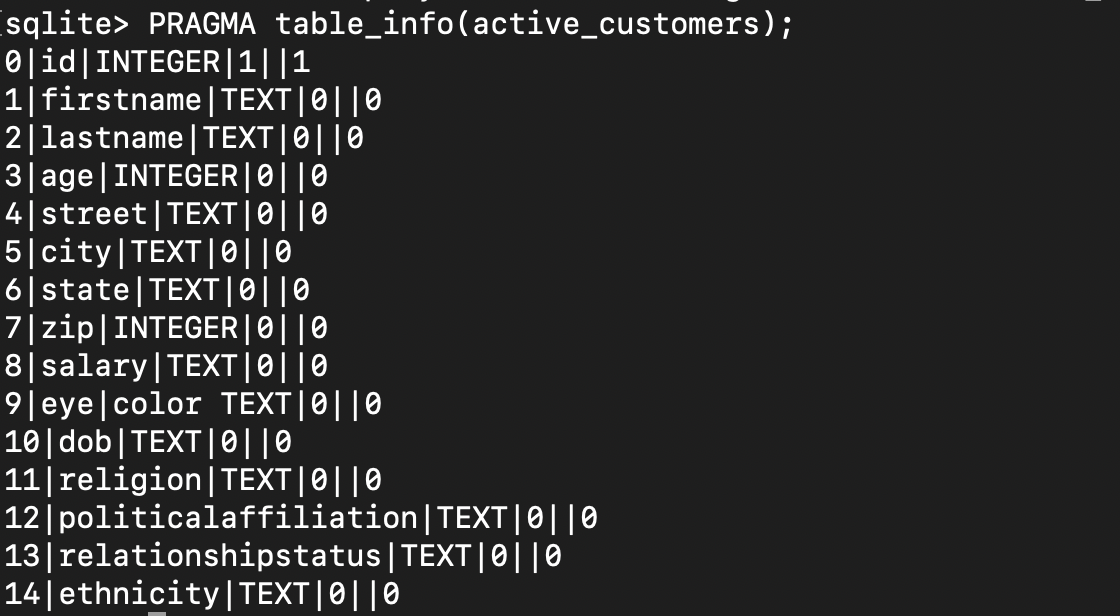
\includegraphics[width=5in]{../images/column-names.png}%
\caption{Table Info}
\label{fig:table info}
\end{figure}
\bigskip
\bigskip

\section{Injection Attack}
\label{sec:injection attack}


When doing the attack, we had to insert SQL queries to try and bypass some
of the log-in administration credentials. With the information that we had gained from
the research of SQL injection attacks, we had done a various number of attacks to try
and inject code into the SQL statements of the web application and gain access to the very sensitive
data that is on the web application. Some examples of things that we did were, we thought
if we were creating a web application, what types of SQL statements would we make to try
and connect the SQL database to the web application to try and make it so that the log-in
credentials would allow someone with the right credentials to log on and see the
information they are allowed to see? When trying to figure out what type of statement
might have been used to connect the database to the site, there were some things that
one could assume were going to be there. First, SELECT username FROM is a good guess as to assuming
what parts of SQL statement would be included since we are dealing with customers and workers
because this is considered to be a banking web application. Stated previously as well, these are also clauses that are common with SQL query statements. Next, we had to try and figure out what may
be on the end of the SQL statement. Well, stated previously, since this is considered to be a banking
web application with log-in credential information, it probably is close to something like, 'username' +
'password'. From here, we can start making some guesses and estimations on what the SQL statement
might look like, but also how we could inject code into this statement to access this data. Again, with the research that we had stated above in the introduction,
there is a lot of common SQL injection code examples that the user could do to bypass a log-in.
With this knowledge, we then started trying different common SQL queries to
gain access. Low and behold, one of the techniques that we had ended up trying actually
worked. This piece of code worked simply because of what it is saying in the SQL query statement. The piece of code was " OR 1=1 --. This worked mainly because of what we were doing. We set the statement to automatically be true. 1=1 is a true statement but the OR in the statement nullifies the SQL query that is proceeding with the statement that we injected. The way it works is like this, imagine we have some sort of random SQL query statement: "SELECT * FROM blah blah blah WHERE blah blah. What we did was we injected SQL code at the end of this query so it would read like this: "SELECT * FROM blah blah blah WHERE blah blah OR 1=1." Ultimately this is negating the first part of the SQL query because the injection is setting everything equal to true. Please see Figure ~\ref{fig:injection attack}

\bigskip
\bigskip
\begin{figure}[hbt!]
\centering
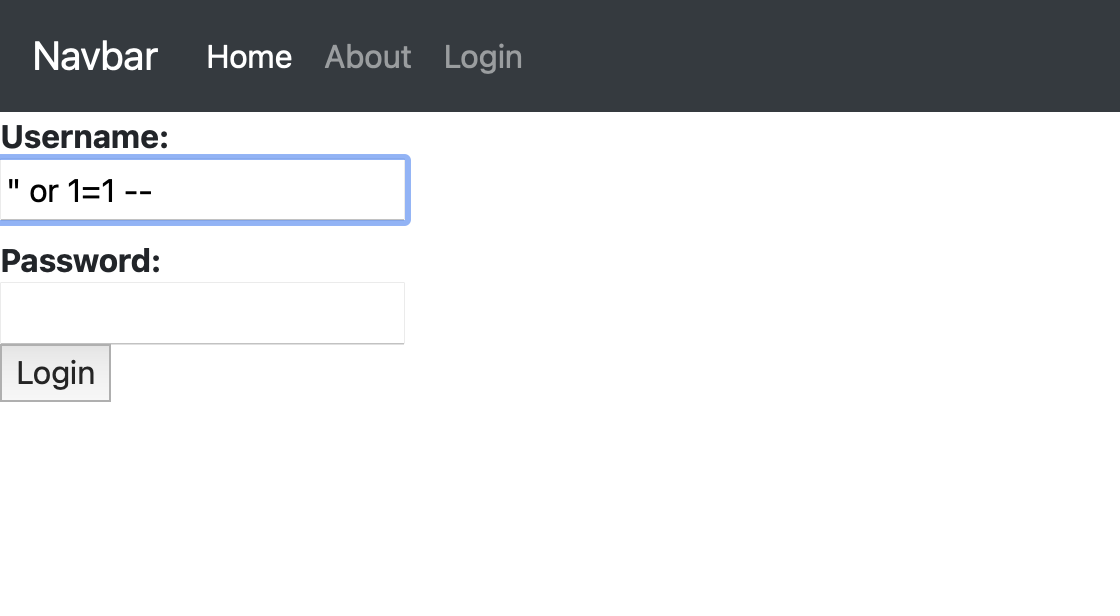
\includegraphics[width=5in]{../images/sql-injection1.png}%
\caption{Injection attack}
\label{fig:injection attack}
\end{figure}
\bigskip
\bigskip

\section{Prototype Implementation}
\label{sec:prototype implementation}


After the SQL injection attack and time permitting, we then started the implementation
for a prototype that allows for better security involving databases. The two main services that we used to help create the prototype were first cloud computing. As we have learned, cloud computing will help with security measures because, cloud computing will allow for the database to not statically sit
on a dedicated server or machine, but it will allow for the database to be accessed
through the cloud. The next service or prototype that we used to implement the prototype was a VPN. From the related work articles, we believed using a VPN helped
with privacy and security as well as it scrambles users' IP addresses and location services so
that the user wouldn't be tracked.

When it comes to the VPN and Cloud computing component of the project, we had to make
sure we could use some sort of software that would allow us to integrate both prototypes.
With much research on this topic, we then concluded using Algo VPN
and digitalOcean cloud computing software. These two prototypes allowed us to set up
a "firewall" of sorts that created an extra layer of security. With the AlgoVPN data
structure, we could create the server and watch and monitor traffic on that
dedicated server ourselves. If anyone tries to access that specific server, we will be
notified. When we paired this with the digitalOcean cloud computing infrastructure, the user will
then be forced to log in to the cloud to access the very sensitive data that
is inside of the database. When the user puts this all together, this is how it should look
like. The first step to access this vital sensitive information would to first
fire up the AlgoVPN and connect to a specific server so that only the user could monitor
the traffic (I.E., no one else knowing where the user is logging onto the database from).
Next, the user can log in to the digitalOcean cloud computing platform and put in the users credentials (
assuming the user has "rights" to view this database). From there, the user should be able to
see the vital information that the user does not want other people to see.


\section{VPN Creation}
\label{sec:vpn creation}


To first start with the implementation of the prototype, we had to first figure
out how to set up the VPN using Algo. With algo, there is a lot of customization.
For starters though, to get going, the user will need to just first download the
required software to do so. We found the documentation from trailofbits.com
And from here we were able to get started. After the user follows the directions, to get
all of the required packages on the users machine up and running one will then need to start up
their virtual environment. For me, I had to go into the algo directory,
then go into the myenv directory, then to the bin directory, and once here, I simply just typed
'source activate' and I was able to start up the virtual environment and get everything running
and underway. Please see Figure ~\ref{fig:virtual environment}

\bigskip
\bigskip
\begin{figure}[hbt!]
\centering
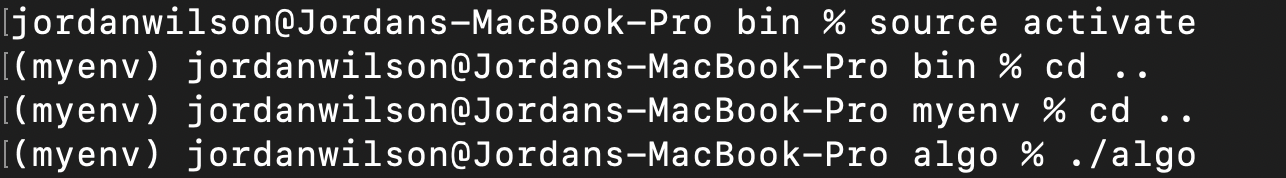
\includegraphics[width=5in]{../images/myenv-1.png}%
\caption{Virtual Environment}
\label{fig:virtual environment}
\end{figure}
\bigskip
\bigskip



After we can get the virtual environment up and running, the next thing we need to
do is start up the algo program to create the VPN. To do that
we simply just type './algo' and the user will then be prompted with a bunch of questions.
The first question that they ask is which cloud provider one would like to use. we had decided
to use DigitalOcean but there are other options such as Amazon EC2, Openstack, Cloudstack,
and others as well. Please see Figure ~\ref{fig:cloud provider}

\bigskip
\bigskip
\begin{figure}[hbt!]
\centering
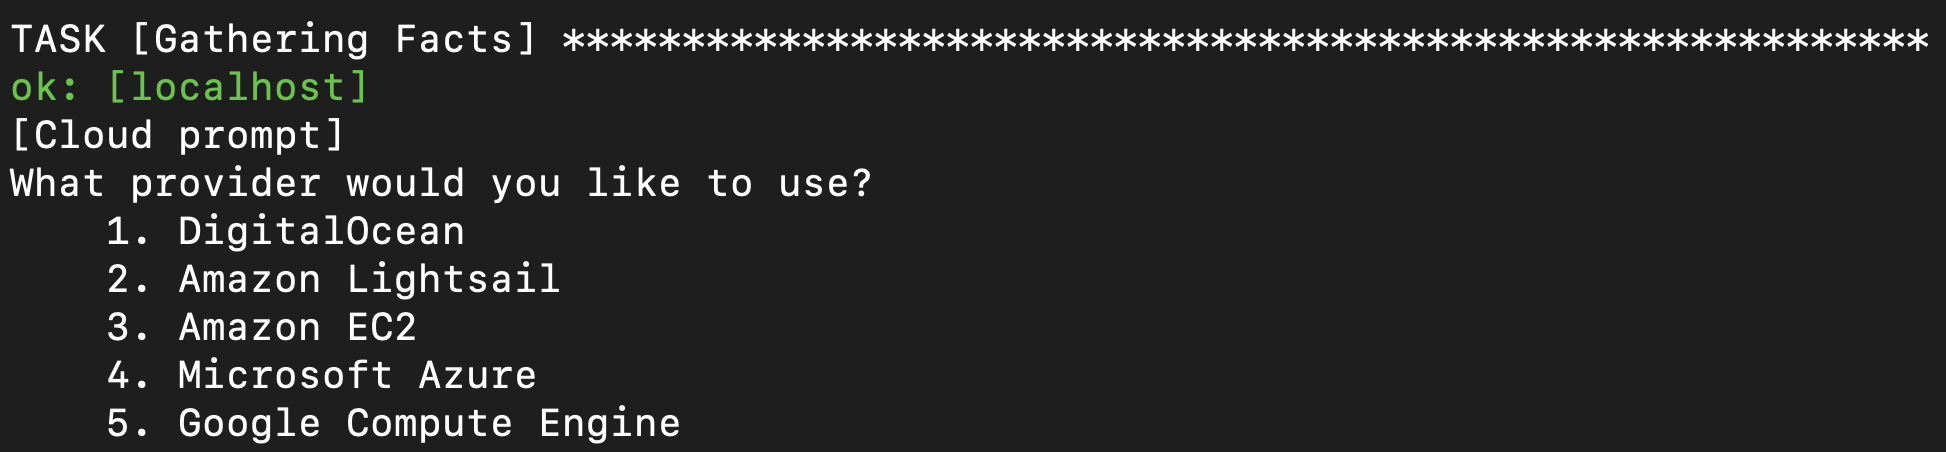
\includegraphics[width=5in]{../images/provider-1.png}%
\caption{Cloud Provider}
\label{fig:cloud provider}
\end{figure}
\bigskip
\bigskip




After the user has chosen which provider they had decided to go with, it then asks the user
a bunch of questions about how to set up the server. It's going to ask the user things
such as VPN server name, if the user wants it to be enabled on clients on-demand for wifi and
cellular networks, names of any trusted wifi networks if one wants to retain any PKI keys,
If the user want to enable DNS blocking on this server, and if the user wants each user of the VPN to have their own
SSH tunneling. From there, it is going to download a few things and then ask the user for their API
token. From there the user will have the option to choose the location of the server, and once that
is down, the user has finally created a VPN. Please see Figure ~\ref{fig:vpn success}



\bigskip
\bigskip
\begin{figure}[hbt!]
\centering
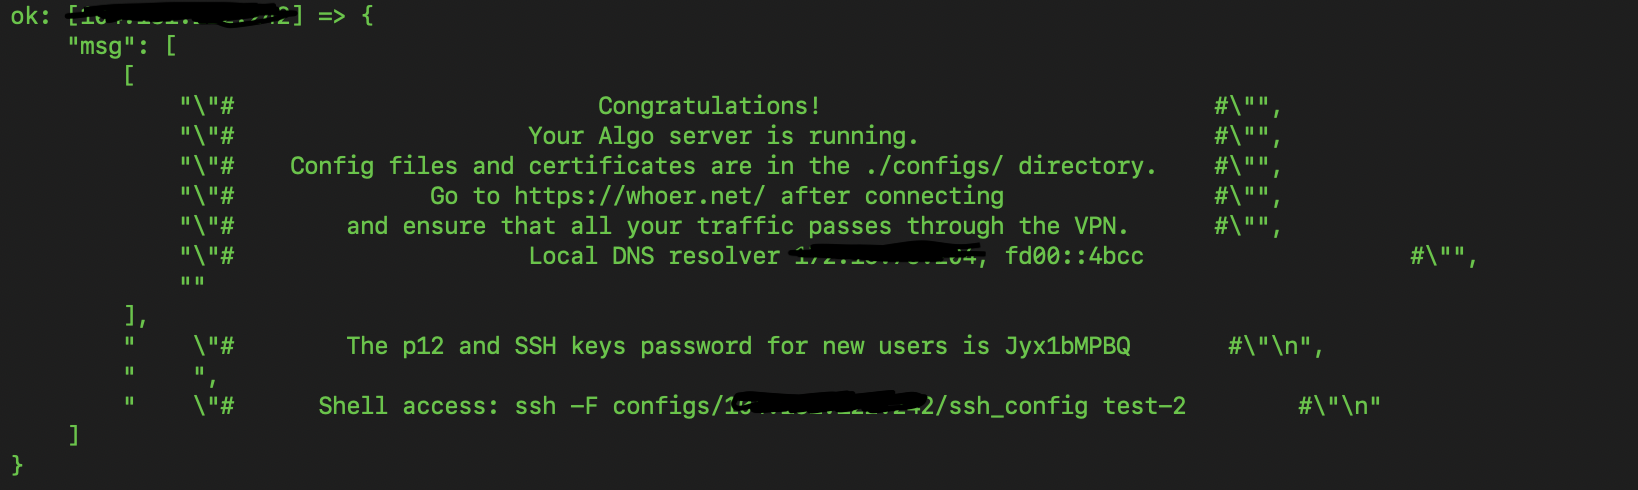
\includegraphics[width=5in]{../images/algo-success1.png}%
\caption{VPN Success}
\label{fig:vpn success}
\end{figure}
\bigskip
\bigskip



From here we now have to access our newly configured VPN. There are a few options available
to us to do that. The options that we have are phone, tablet, and laptop. Personally,
I had decided to set it up on my phone. Once we are greeted with the congratulations
page that our VPN is set up, it also gives us a web application that we have to go to to make sure our new IP address is masked. The web application is whoer.net and we'll just keep
this there for reference right now. To use the VPN on a device, we
have to have wireguard VPN installed. This will allow us to connect to our server. Once we have
wireguard installed, it will let us add a new connection at the top right of the screen.
From there, we can name our new connection and then actually connect to it. There are two different
ways the user can connect to the server through wireguard, but the easiest way and the way that we did
it was to simply use the barcode that is in our algo files. This will allow for easy
connectivity for us to connect to the server. Once we had located the phone barcode
picture, we then just went back on my phone and scanned the barcode and we then were
easily able to connect to the VPN server! After we had done this, we then went
back to the whoer.net web application we had referenced earlier and we were able to see that I
was connected to a different server and the IP address was indeed masked. Please see Figure ~\ref{fig:vpn access}



\bigskip
\bigskip
\begin{figure}[hbt!]
\centering
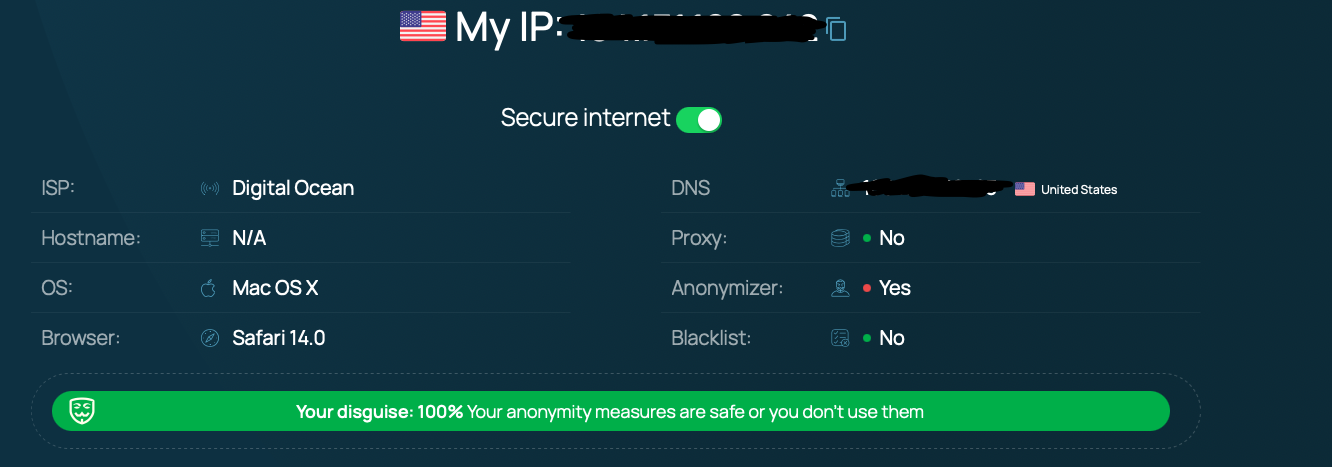
\includegraphics[width=5in]{../images/whoer-1.png}%
\caption{VPN Access}
\label{fig:vpn access}
\end{figure}
\bigskip
\bigskip
\bigskip
\bigskip


\section{Cloud Database Cluster}
\label{sec:cloud database cluster}


After the completion of the VPN server, we now could move onto creating the cloud virtual
server to create a database and access it. For this part, we used DigitalOcean
almost exclusively. The first big step we did to create the databases through
DigitalOcean was that we needed to purchase a database cluster from DigitalOcean.
With DigitalOcean, there come subscriptions that the user will have to pay for to
use their services which is unfortunate, but their services do make what we were trying to
do a bit easier. After we had purchased a database cluster, we then start picking and choosing
what options we am going to need. In digitalOcean there are a few different engines the user can
use. The options are PostgreSQL, MySQL, and Redis. For this project, we decided to
use Redis. The next option the user has is how large one would want their node size to be. For this
option though, the user has to be careful because the bigger the node size, the more money
they will have to pay a month for this cluster. The next thing the user has to choose is
a data center. For convenience, we decided to go with New York since that is close to where
we am and it will take less time connecting to the database cluster but other options
the user can choose from are Amsterdam, San Francisco, London, and Singapore just to name a few.
After the user has chosen their desired settings, all one has to do now is come up with a unique
database cluster name. Please see Figure ~\ref{fig:mysql connection}



\bigskip
\bigskip
\bigskip

\bigskip
\begin{figure}[hbt!]
\centering
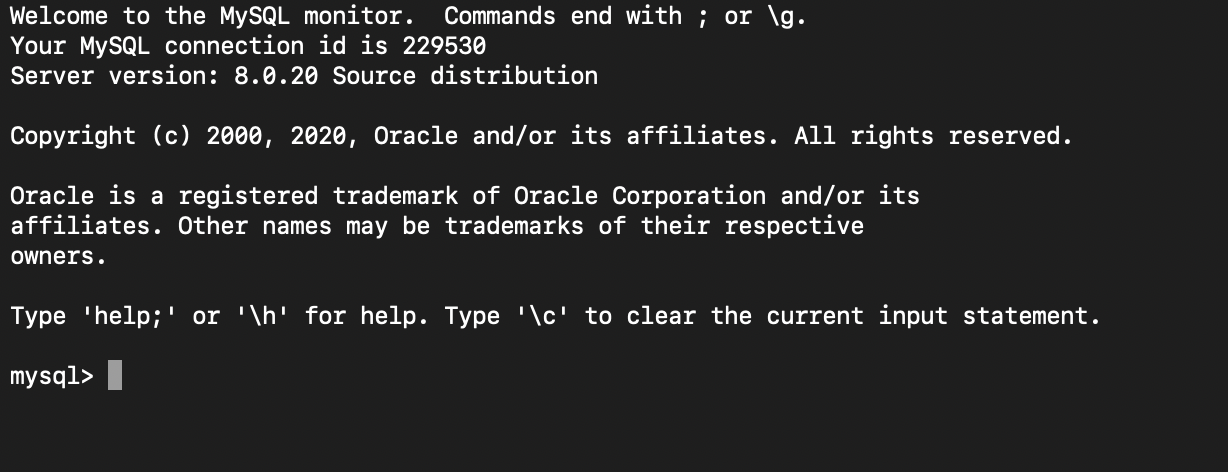
\includegraphics[width=5in]{../images/mysql-terminal.png}%
\caption{MySQL Connection}
\label{fig:mysql connection}
\end{figure}
\bigskip




After the creation of the users database cluster, one has to set some preferences as well.
A big preference one has to set is their trusted sources. This is super vital to this
project. This is how we will integrate the VPN and the database cluster. What I
did was I set the trusted sources to only it being the VPN IP that we had created earlier.
With this, I am able to only access this database cluster when I am connected to a specific
VPN server that I (or the user) have created. This just adds an extra layer of security.
After the user chooses their trusted sources and fill out the rest of the information that one
would like, digitalOcean will provide the user with their connection parameters, and from here
one can connect to the database cluster. Please see Figure ~\ref{fig:mysql databases cluster}


\bigskip
\bigskip

\begin{figure}[hbt!]
\centering
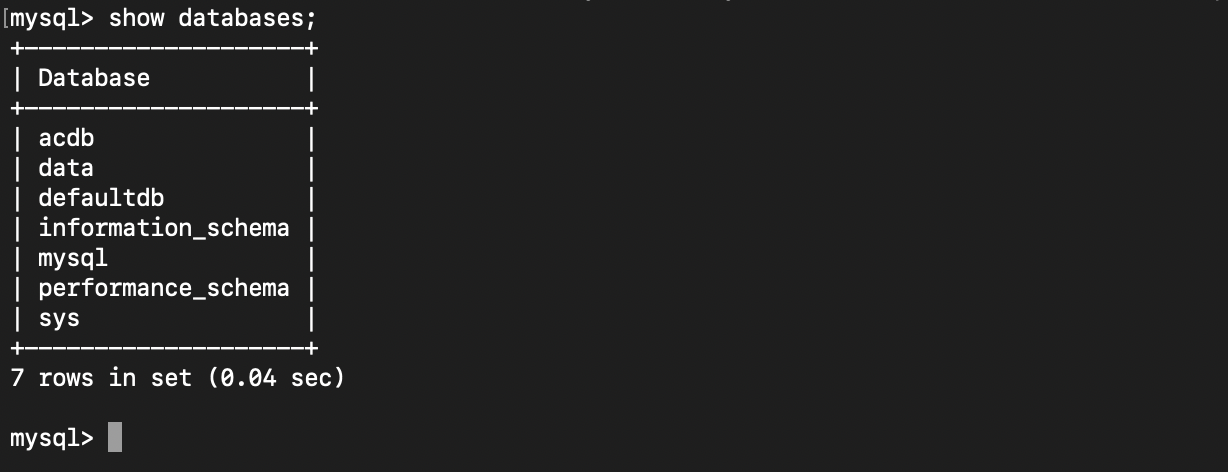
\includegraphics[width=5in]{../images/mysql-db.png}%
\caption{MySQL Databases Cluster}
\label{fig:mysql databases cluster}
\end{figure}







%\numberedchapter{Experimental Results}
\chapter{Experimental Results}
\label{ch:experiments}

\section{Experimental Design}

For this project, my experimental design revolves around the fact that we are bypassing
a login screen and with that, being able to gain access to a large quantity of data that
consists of variables such as firstname, lastname, age, salary, eye color, ethnicity
as well as a few other factors. The way that the experiment had been set up was by first
researching a lot about the topic. SQL injection is a very popular injection technique
so there is a lot of documentation out there on the subject. Another big point was figuring out how to exactly inject the SQL code to
bypass the log-in. While initially thinking about this, it had sounded much more
complicated, but once we had researched and planned out what needed to happen, things
started coming together. The experiment here was seeing if not only could it be possible to create a database and web application but bypass
the login with just some SQL query statements. From the introduction, there was talk about
the different possible SQL query statements that are common to try and bypass a login
that is associated with web applications. Since we are trying to figure out why this
might have been the case though, and we thought that it would be best to try and look at the code to try and figure out
why this might be the case. So for here, the starting point would be the SQL
query statement that is used to connect the web application and the database. For this
particular project, one would not only have to come up with a query statement that will connect
the two but also come up with a piece of code that one can inject into my SQL query statement.
Let us start one step at a time though. To connect the database and the web application
with the query statement, one would have to give it the parameters that are necessary so it will choose
the right table, and display all of the information that is desired if it has the proper
login credentials. If it doesn't then it will just redirect to a different page. With this
knowledge, we now must figure out the best query statement to connect the two. This
is what we came up with.


\bigskip
\bigskip
\begin{lstlisting}
cur = g.db.execute("select username from managers where username=\""+request.form['username']+"\""+"and password=\""+request.form['password']+"\"")
\end{lstlisting}
\bigskip
\bigskip


\section{Evaluation}

Based on this query, and the SQL injection piece of code that had been shown earlier, we
can bypass the login and see all of the important data. Everything
that is in the database will also be displayed to us. One could say based on us being
able to do that, The evaluation of my experiment went pretty well. We had predicted
that one could bypass the log-in if the user knew what the SQL query statement was and since
we created it, we of course knew what it was. These are the results below. As you can see the id for web application and for the database are the same meaning the database associated with each is the same, the difference is how each were accessed.

\bigskip
\bigskip
\begin{figure}[hbt!]
\centering
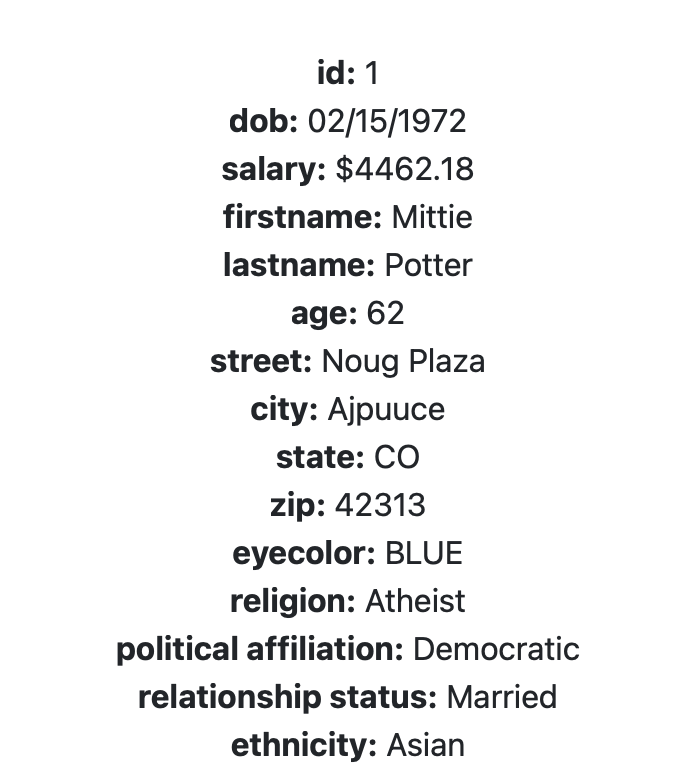
\includegraphics[height=3in]{../images/access-1.png}%
\caption{Data on Website}
\label{fig:data on website}
\end{figure}
\bigskip

\bigskip
\begin{figure}[hbt!]
\centering
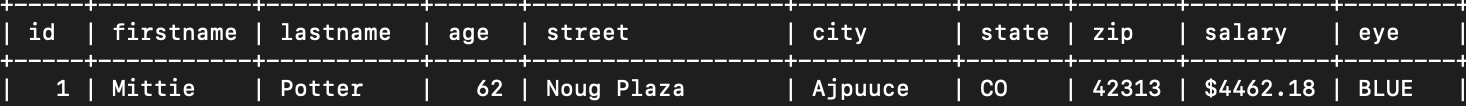
\includegraphics[width=6in]{../images/access-2.png}%
\caption{Data in Terminal}
\label{fig:data in terminal}
\end{figure}
\bigskip
\bigskip



\section{Threats to Validity}

There could be arguments with the validity of my work. One could argue
that for my SQL injection code, I made it so that whatever was had put in the username
column would be in the username column in my database. Ultimately making it just
log me in instead of bypassing the login. Another argument could be that
I didn't create the VPN and database cluster together, meaning that you don't necessarily have to connect to the VPN to connect to the database. This of course
though, is false. Certain trusted servers allow the database to be logged
into from. The way that I had set it up is that you have to be connected
to a specific server to be able to log in, and in my case, it is the server
that we are connected to through our VPN. There may be more claims as to what are
other threats to validity, but with the work that I have done and everything I was
able to complete, I believe my work stands solid. A big point for validity though is the notion
that an SQLite database was used to store the data that is associated with the web application. This could be considered a threat because SQLite databases are not as robust as industry-standard ones such as MySQL and PostgreSQL. The industry-standard ones have better security so by-passing a log in the way that was demonstrated wouldn't be as easy as it seems. The idea though is still the same. MySQL is not the end-all-be-all-perfect database that has no security issues so my point still stands solid. Security associated with web applications and databases needs to be improved upon and better.

%\numberedchapter{Conclusion}
\chapter{Discussion and Future Work}
\label{ch:conclusion}

\section{Summary of Results}

From the graphs and data that we can see throughout the document. I think it is
safe to say that this type of injection technique is very prominent throughout
the cybersecurity world. Having the ability to bypass a login because of sloppy code
that is written to connect a database to a web application is pretty important. Not
only that but we can see how damaging something like this can be. Not only from the examples
that were given in the introduction but also from the way we walked through the
process of how one can do this. We can see that this type of technique can
work. Along with that, we can see that the proposed prototype that I had decided to
work on also looks very promising. As one can see the user can set up a
database that is in the cloud, and only have it accessible if you have the right credentials. The
way we set it up as one can see is that there are multiple layers of security so you can't
just try to bypass some type of security protocol and expect to automatically get the
important and sensitive data. Being able to only access the database with certain
criteria and showing that the data that is both stored on the website and through the
database cluster through the cloud both show good examples of how this prototype can work.
From a look at the results, I think it is safe to say that the proposed prototype
looks like it could be a promising prototype that mitigates vulnerabilities that are associated
with web applications and databases.

\section{Ethics}

A really big key point of this project was the ethical implications surrounding it. The idea behind this project was to not only show how there are security issues surrounding databases associated with web applications but also talk about why someone may try to use a certain technique to gain access to information they are not supposed to see. Here lie the ethical implications surrounding my very topic. One may have the ability to gain access to very sensitive information but does that mean they should do it? When we take a look at the data of the project each "id" represents another human being. Human beings have rights and a big right that they have is the right to privacy and security. This project should not tell you to go out and to try and "hack" different websites. This project is aimed at showing you the ethical implications that surround hacking. However, there are a few ethical reasons as to why someone may try and use techniques such as the one that has been demonstrated. For example, there are certain jobs out there that do ethical hacking. White Box Testing that was described earlier is an example of ethical hacking. What does this look like though? Well, people who work for consulting firms can be hired to try and hack a companies website. This is to try and find out if their sites have any vulnerabilities that they can find and if they can, they will report back with their findings. This will allow companies to continue to improve their security when it comes to important things like websites and databases. This is just an example to show you that there are ethical reasons for hacking. The sad truth of this story though is hacking is used more for unethical reasons. Stealing data, leaking classified information, and deleting important information are all examples of ways people have used hacking techniques unethically. 

\section{Importance}

This type of work is very important. What I have done in this project, is that I have shown that you can access very private information on a web application very easily. People's whole lives are just an id number in databases that are stored online on companies' websites and this can be a problem when the right security measures aren't being taken. This work is showing that there are security issues that have been found, but nobody has gone back to fix these issues. SQL injection is one of the major issues associated with attacking data on web applications so why hasn't this problem been fixed if it has been around since the early 2002's? These are the types of questions I hope to find answers to as I do more research and learn more about security that revolves around databases. MySQL, for example, is more of an industry-standard database most companies use rather than SQLite so the security around that database is better, but it still is not full proof to safeguard against attacks. Lots of people around the world are putting their trust in major companies such as Amazon, Apple, and Microsoft. Yet, Companies like Facebook and Yahoo have had major data breaches and lost the trust of so many of their users. This project aims to continue the ongoing research and development of the best security methods to ensure people's privacy. If major companies like those continue to lose the trust of their users because of breaches our economy will also plummet. Imagine a world where Amazon has been hacked and no one trusts to use their services anymore. Our way of life in terms of receiving packages would completely change.


\section{Conclusion}

With the completion of this project. There were a lot of big key takeaways, not
only from the technical standpoint of security involved with computer science but
also the ethics that are involved with people giving their information away to companies
and companies storing them in a big database. Everyone should not have to give away
so much of their information to create an account with a company. I purposefully chose
the variable that I did to show that if a major company or corporation had a data
breach. Lots of people's information would just be out and the type of information that
sits in those databases are people's lives. When I look at each id in that database, I see a person. Since that id represents another human-being we have to
be very diligent and precise when we are thinking about putting data in a database
that can be accessed online. To me, there isn't enough security in the world to ensure
that the data in the database is secured. It represents a person's whole life. I believe
a project like this should prompt companies and organizations to re-think the types
of requirements that are necessary to open an account with them.

\section{Future Work}

There is a lot of future work that can be done for this project. The further implementation
of my prototype is something that should continue to be worked on as it will
help uncover other possible security vulnerabilities that are related to data and databases
online. With the start of the implementation of my prototype, however, there were numerous
things that I learned that I think are very helpful when it comes to putting sensitive
data in a database. One important thing is that the cloud computing aspect of this
makes this a lot easier as well. When you put data on a database and you connect it
to a web application, essentially your database is just sitting on the same server
being stagnant. With the cloud computing aspect, your database is not stagnant on a  single server, so you just can choose which servers can access that database. This will complicate things
a little because this messes with the client-host server details which are a bit
different from having a database connected to a web application. Another big detail is
the fact that you can make accessing data in a database using a VPN a PRIORITY. This can be extremely helpful when
accessing sensitive data online because then, no one would know where you are originally
signing in from. You are masking your actual IP address so this will make tracking you
and your location much difficult, not to mention this will also make it much more
difficult for hackers to try and figure out what server your database can be accessed
through. As regarding plans for this type of project though, I think something
that should be looked at is implementing this associated with a web application in
some way. If, somehow, we could create a web application page that will redirect the
user to a cloud computing machine and then from there, try to login with the credentials
to try to access the data in the database that would be a step in the right direction. As well, if the user is not connected to that
specific IP address that is in tangent with the VPN associated with the database cluster
then the user should not be able to see any information and if the user is connected to
the proper IP then the user should be granted access.





%----------------------------------------------------------------------------------------
%	BIBLIOGRAPHY
%----------------------------------------------------------------------------------------

\addtocontents{toc}{\vspace{2em}} % Add a gap in the Contents, for aesthetics
\unnumberedchapter{Bibliography} % Title of the unnumbered chapter
\bibliography{preamble/bibliography} % The references information are stored in the file named "bibliography.bib"


\end{document}
